\documentclass{ieeeaccess}
%Adjusted 05/13/2026 at the byline author names
\usepackage{cite}
\usepackage{amsmath,amssymb,amsfonts}
\usepackage{algorithmic}
\usepackage{algorithm}
\usepackage{graphicx}
\usepackage{textcomp}
%\usepackage{caption}
%\usepackage{subcaption}
%\usepackage{algpseudocode}
\usepackage{enumerate}
\usepackage{siunitx}
\usepackage{comment}
\usepackage{capt-of}  % For \captionof command


\usepackage{bm}
\makeatletter
\AtBeginDocument{\DeclareMathVersion{bold}
\SetSymbolFont{operators}{bold}{T1}{times}{b}{n}
\SetSymbolFont{NewLetters}{bold}{T1}{times}{b}{it}
\SetMathAlphabet{\mathrm}{bold}{T1}{times}{b}{n}
\SetMathAlphabet{\mathit}{bold}{T1}{times}{b}{it}
\SetMathAlphabet{\mathbf}{bold}{T1}{times}{b}{n}
\SetMathAlphabet{\mathtt}{bold}{OT1}{pcr}{b}{n}
\SetSymbolFont{symbols}{bold}{OMS}{cmsy}{b}{n}
\renewcommand\boldmath{\@nomath\boldmath\mathversion{bold}}}
\makeatother

\def\BibTeX{{\rm B\kern-.05em{\sc i\kern-.025em b}\kern-.08em
    T\kern-.1667em\lower.7ex\hbox{E}\kern-.125emX}}


%Your document starts from here ___________________________________________________
\begin{document}
\history{Date of publication xxxx 00, 0000, date of current version xxxx 00, 0000.}
\doi{10.1109/ACCESS.2024.0429000}

\title{Preparation of Papers for IEEE ACCESS}
\author{\uppercase{First A. Author}\authorrefmark{1}, \IEEEmembership{Fellow, IEEE},
\uppercase{Second B. Author}\authorrefmark{2}, AND \uppercase{Third C. Author},
Jr.\authorrefmark{3},
\IEEEmembership{Member, IEEE}}

\address[1]{National Institute of Standards and
Technology, Boulder, CO 80305 USA (e-mail: author@boulder.nist.gov)}
\address[2]{Department of Physics, Colorado State University, Fort Collins,
CO 80523 USA (e-mail: author@lamar.colostate.edu)}
\address[3]{Electrical Engineering Department, University of Colorado, Boulder, CO
80309 USA}
\tfootnote{This paragraph of the first footnote will contain support
information, including sponsor and financial support acknowledgment. For
example, ``This work was supported in part by the U.S. Department of
Commerce under Grant BS123456.''}

\markboth
{Author \headeretal: Preparation of Papers for IEEE TRANSACTIONS and JOURNALS}
{Author \headeretal: Preparation of Papers for IEEE TRANSACTIONS and JOURNALS}

\corresp{Corresponding author: First A. Author (e-mail: author@ boulder.nist.gov).}


\begin{abstract}
Current development of microservice architectures heavily relies on API gateways and high-performance RPC frameworks like gRPC, the implementation details of the inter-service communication layer are often abstracted away in system design. Our paper empirically investigates the performance degradation caused by application-layer communication bottlenecks, with particular focus on gRPC connection management. We present a mathematical queueing model and algorithmic formalization to quantify the overhead of the connection-per-request (CPR) compared to a persistent channel reuse (PCR). Our evaluation results in Kubernetes environment tests show that converting CPR to PCR models can significantly reduce median latency by 97\%—from over 7,000 ms to 150 ms under peak load. This change significantly eliminates the performance bottleneck that caused an increase in end-to-end user experience latency time.
\end{abstract}

\begin{keywords}
Cloud-Native, Connection Per Request, gRPC API, High Performance Computing, Kubernetes, Microservices, Persistent Channel Reuse 
\end{keywords}

\titlepgskip=-21pt

\maketitle


%%%%%%%%%%%%%%%%%%%%%%%%%%%%%%%%%%%%%%%%%%%%%%%%
\section{Introduction}
\label{sec:intro}
%%%%%%%%%%%%%%%%%%%%%%%%%%%%%%%%%%%%%%%%%%%%%%%%

\begin{comment}
\PARstart{T}{he} transition to cloud-native microservices has established API gateways and high-performance RPC frameworks like gRPC as standard infrastructure. In this architecture, the API gateway functions as the singular entry point for external traffic, acting primarily as a reverse proxy and protocol transcoder. While external clients typically communicate using standard HTTP/1.1 and JSON payloads—often following RESTful paradigms as discussed in \cite{martin2022online}—internal microservices increasingly rely on gRPC over HTTP/2 for high-performance communication \cite{Ventre2018SDNAAA}. Unlike the stateless nature of traditional REST, gRPC is specifically designed to multiplex many requests over a single persistent HTTP/2 connection. However, the implementation details of this inter-service communication layer are often abstracted away by frameworks. As study by \cite{zhu2023dissecting}, have exposed significant infrastructural overheads hidden within service mesh sidecars, we observe that analogous, undocumented performance penalties exist within the application layer of API gateways when protocol translations are mismanaged.

The specific issue addressed in this paper is the performance degradation caused by the "connection-per-request" (CPR) anti-pattern within these gateways. Previous studies have shown how TCP and TLS handshake delays reduce throughput in distributed systems \cite{Guo2020StatefulTCPANAA}. However, the direct application of legacy REST-based connection management to gRPC environments remains a pervasive flaw. We define gRPC connection churn as the continuous cycle of establishing and tearing down complex network state (TCP handshakes and HTTP/2 protocol negotiations) for every individual application-layer request, rather than multiplexing traffic. Establishing a new connection per request is an $O(N)$ operation, where $N$ represents the number of incoming client requests. This directly conflicts with the $O(1)$ multiplexed design of HTTP/2, forcing gateway worker threads to spend excessive CPU cycles on network context switching. We explore this vulnerability using a standard Python WSGI stack \cite{wsgi-pep} (Flask and Gunicorn) as a representative testbed, as its synchronous worker model clearly exposes the severe latency penalties of blocking network I/O.

While the research community has modeled microservice performance extensively, the specific intersection of application-layer connection churn and queueing network saturation remains empirically unquantified. Recent academic works, such as those by Pinheiro et al. \cite{pinheiro2024performance}, utilize stochastic Petri Nets to evaluate microservice resilience; however, evaluating latency under load requires a shift toward queueing theory. We argue that bottlenecks at the implementation level, particularly the phenomenon of gRPC connection churn, lead to a dynamic increase in the service time ($S$) of the system. In queueing theory \cite{DAuria2021AnMQA}, an inflated service time severely degrades the theoretical service rate ($\mu$). This churn converts what should be a constant-time RPC execution into a highly variable, load-dependent event. Previous research has not addressed how this specific application-layer mismanagement forces premature queue saturation long before physical CPU or memory limits are reached.

Therefore, this paper demonstrates how converting the original CPR approach into a Persistent Channel Reuse (PCR) approach, as shown in the Fig. \ref{fig1}—by refactoring the gateway code to initialize a global, thread-safe gRPC channel at startup—eliminates this bottleneck. To validate this, the specific contributions of this paper are as follows:

\begin{itemize}
    \item We model the request patterns and application-layer logic based on both the CPR and the refactored PCR approaches.
    
    \item We introduce a queueing-theoretic model to explain the non-linear latency spikes observed under high load, linking application-layer connection churn to queue saturation.
    
    \item We benchmark these models within an actual Kubernetes environment using controlled isolation environment—\break{ensuring} the gateway is evaluated independently of backend database or business logic variance—to validate the correctness of the theoretical model against empirical runs.
\end{itemize}

\begin{figure*}[t!]
	\centering
	
	\begin{minipage}{0.45\textwidth}
		\vspace*{0pt}
		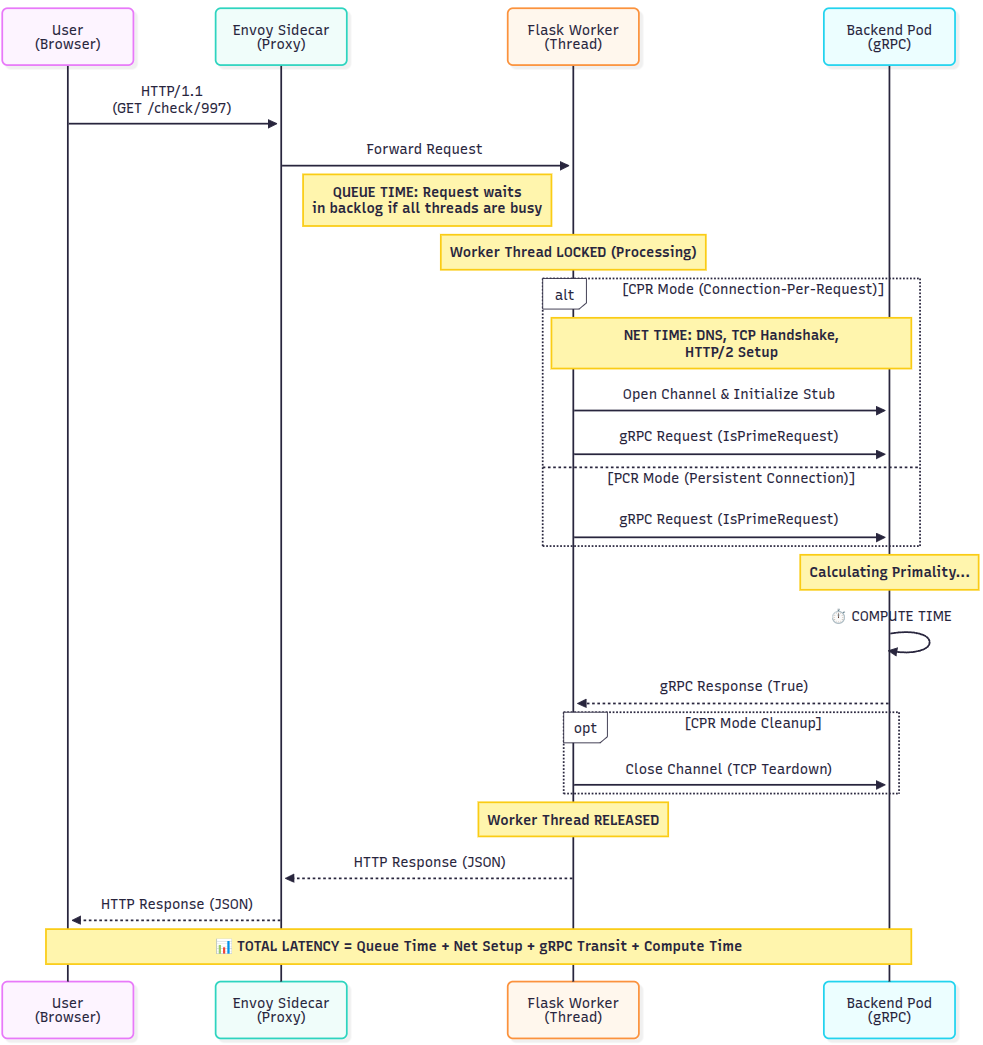
\includegraphics[scale=0.26]{fig/seq-diagram-1-sync.png}
		%\vspace*{4pt}
		\centering{\small(a)}
		\label{fig:sync}
	\end{minipage}
	\hfill
	\begin{minipage}{0.48\textwidth}
		\vspace*{0pt}
		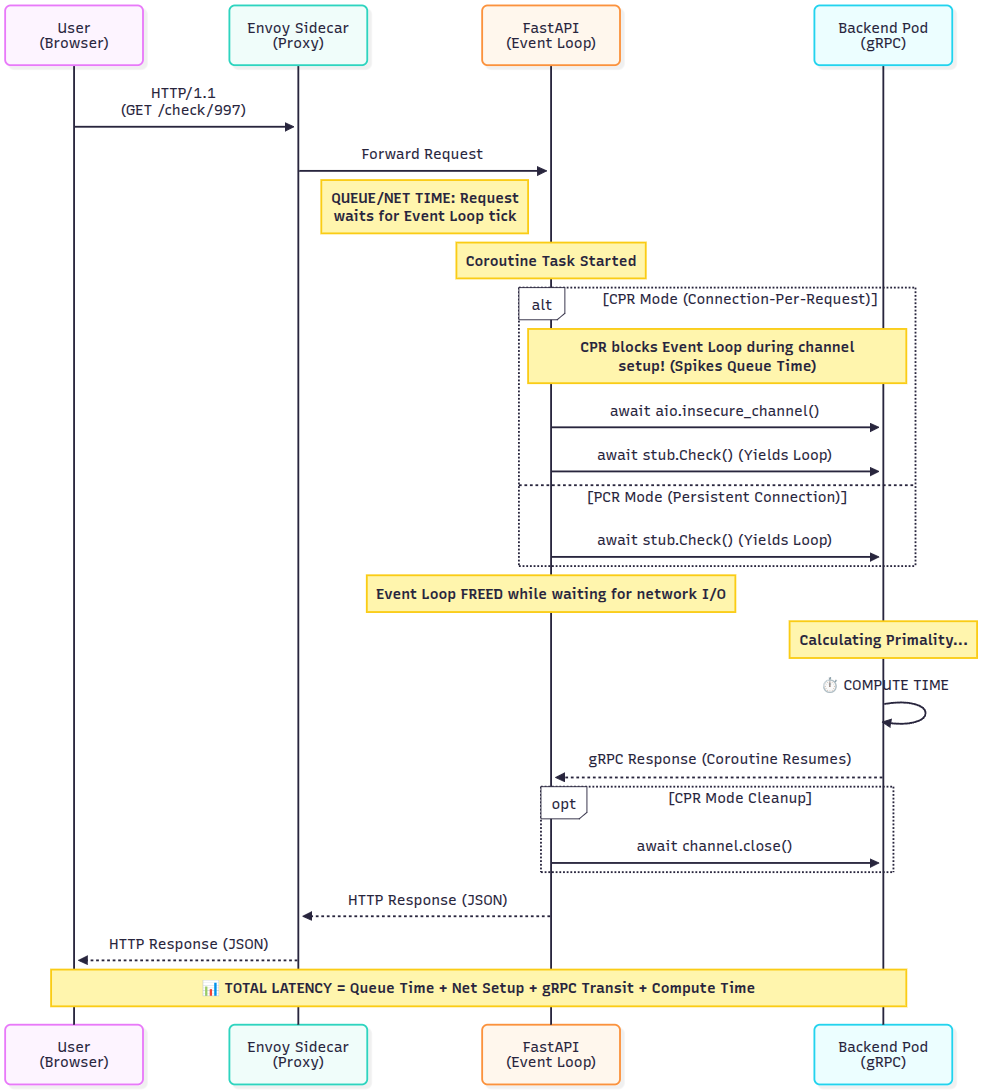
\includegraphics[scale=0.25]{fig/seq-diagram-2-async.png}
		%\vspace*{4pt}
		\centering{\small(b)}
		\label{fig:async}
	\end{minipage}
	%\vspace{10pt}
	\caption{\textbf{Sequence process of synchronous vs asynchronous communication models of cloud-native application on Connection Per Use (CPR) and Persistant Connections Reuse (PCR): (a) Synchronous CPR/PCR (Flask/Gunicorn); (b) Asynchronous CPR/PCR (Flask/Uvicorn).}}
	\label{fig:seq-model}
\end{figure*}

\end{comment}


\PARstart{T}{he} transition to cloud-native microservices has established API gateways and high-performance RPC frameworks like gRPC as standard infrastructure. In this architecture, the API gateway functions as the singular entry point for external traffic, acting primarily as a reverse proxy and protocol transcoder. While external clients typically communicate using standard HTTP/1.1 and JSON payloads—often following RESTful paradigms as discussed in \cite{martin2022online}—internal microservices increasingly rely on gRPC over HTTP/2 for high-performance communication \cite{Ventre2018SDNAAA}. Unlike the stateless nature of traditional REST, gRPC multiplexes multiple requests over a single persistent HTTP/2 connection. However, the implementation details of this inter-service communication layer are often abstracted away by frameworks. As demonstrated by Zhu et al. \cite{zhu2023dissecting}, significant infrastructural overheads remain hidden within service mesh sidecars; similarly, we observe that undocumented performance penalties exist within the application layer of API gateways when protocol translations are mismanaged.

The specific issue addressed in this paper is the performance degradation caused by the "connection-per-request" (CPR) anti-pattern within these gateways. Previous studies have shown how TCP and TLS handshake delays reduce throughput in distributed systems \cite{Guo2020StatefulTCPANAA}. However, applying legacy REST-based connection management to gRPC environments remains a pervasive flaw. While recent work on high-throughput serialization formats like Bebop highlights how CPU branch mispredictions and framing overheads bottleneck RPC runtimes \cite{sampson2026simplicity}, the fundamental overhead of connection instantiation at the gateway level is frequently overlooked. We define gRPC connection churn as the continuous cycle of establishing and tearing down complex network state (TCP handshakes and HTTP/2 protocol negotiations) for every individual application-layer request, rather than multiplexing traffic. Establishing a new connection per request is an $O(N)$ operation, where $N$ represents the number of incoming client requests. This directly conflicts with the $O(1)$ multiplexed design of HTTP/2, forcing gateway worker threads to spend excessive CPU cycles on network context switching. We explore this vulnerability using a standard Python WSGI stack \cite{wsgi-pep} (Flask and FastAPI) as a representative testbed, as its synchronous worker model clearly exposes the severe latency penalties of blocking network I/O.

While the research community has modeled microservice performance extensively, the specific intersection of application-layer connection churn and queueing network saturation remains empirically unquantified. Recent works evaluate microservice resilience using stochastic Petri Nets \cite{pinheiro2024performance} or optimize multi-service resource provisioning using stochastic execution models \cite{carnevali2025compositional}. However, evaluating dynamic latency under load requires integrating these approaches with queueing theory \cite{DAuria2021AnMQA}. We argue that implementation-level bottlenecks, specifically gRPC con-nection churn, dynamically inflate the service time ($S$) of the system, degrading the effective service rate ($\mu$). This churn converts what should be a constant-time RPC execution into a highly variable, load-dependent event. Unmanaged connection churn destabilizes base duration estimates, forcing premature queue saturation long before physical CPU or memory thresholds are reached.

Therefore, this paper demonstrates how converting the CPR model into a Persistent Channel Reuse (PCR) model, as illustrated in Fig. \ref{fig:seq-model}, eliminates this bottleneck by refactoring the gateway code to initialize a global, thread-safe gRPC channel at startup. To validate this approach, the key contributions of this paper are as follows:

\begin{itemize}
	\item We formalize and model the request patterns and application-layer execution logic for both the CPR and refactored PCR models.
	
	\item We introduce a queueing-theoretic model to explain non-linear latency spikes under high load, establishing a direct link between application-layer connection churn and queue saturation, thereby yielding a proposed controller that continuously senses for any change of catastrophic bottleneck to the frontend application.
	
	\item We benchmark these models within a production Kubernetes cluster using controlled and isolated environment, ensuring the gateway of both frontend and backend business logic variance is independently evaluated, to validate theoretical queueing projections against empirical execution runs.
\end{itemize}

\begin{figure*}[t!]
	\centering
	\begin{minipage}{0.48\textwidth}
		\centering
		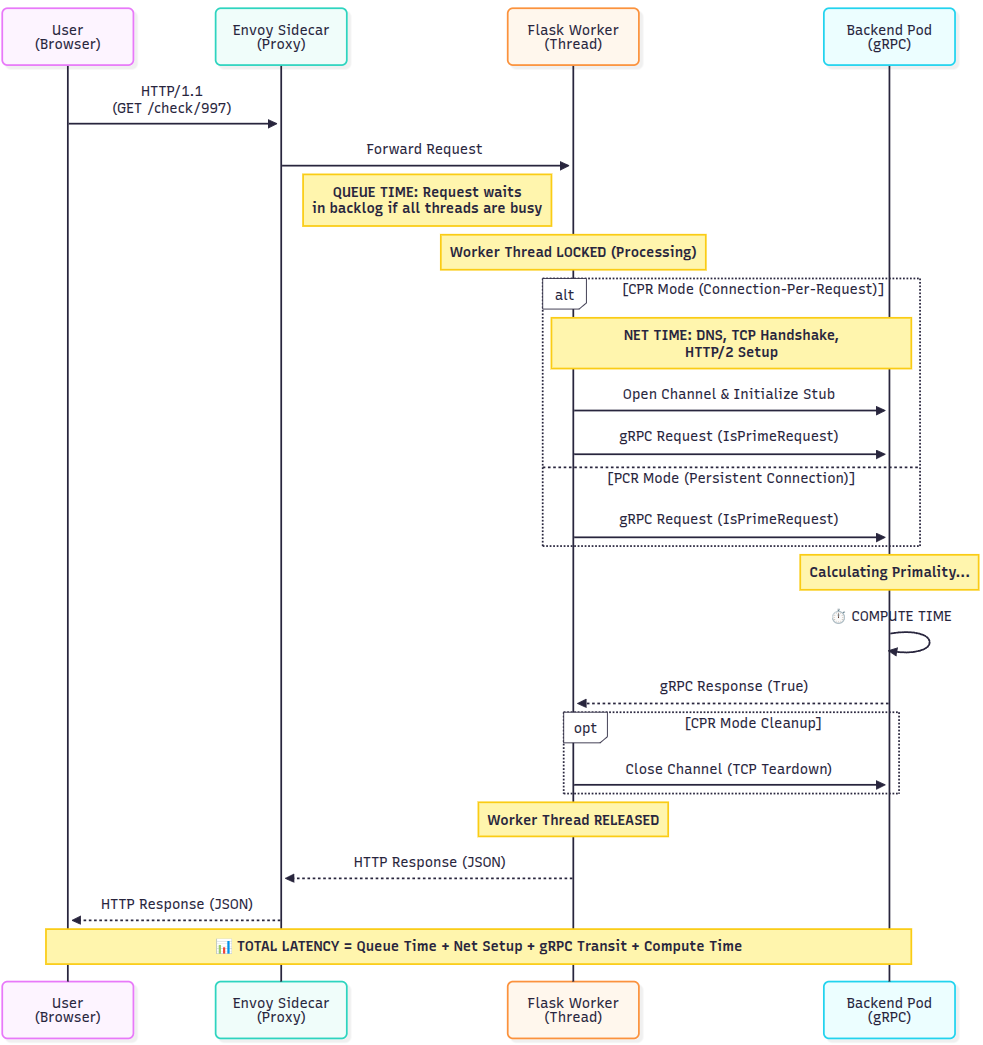
\includegraphics[width=\textwidth]{fig/seq-diagram-1-sync.png}
		\vfill
		{\small  (a)}
		\label{fig:sync}
	\end{minipage}
	\hfill
	\begin{minipage}{0.47\textwidth}
		\centering
		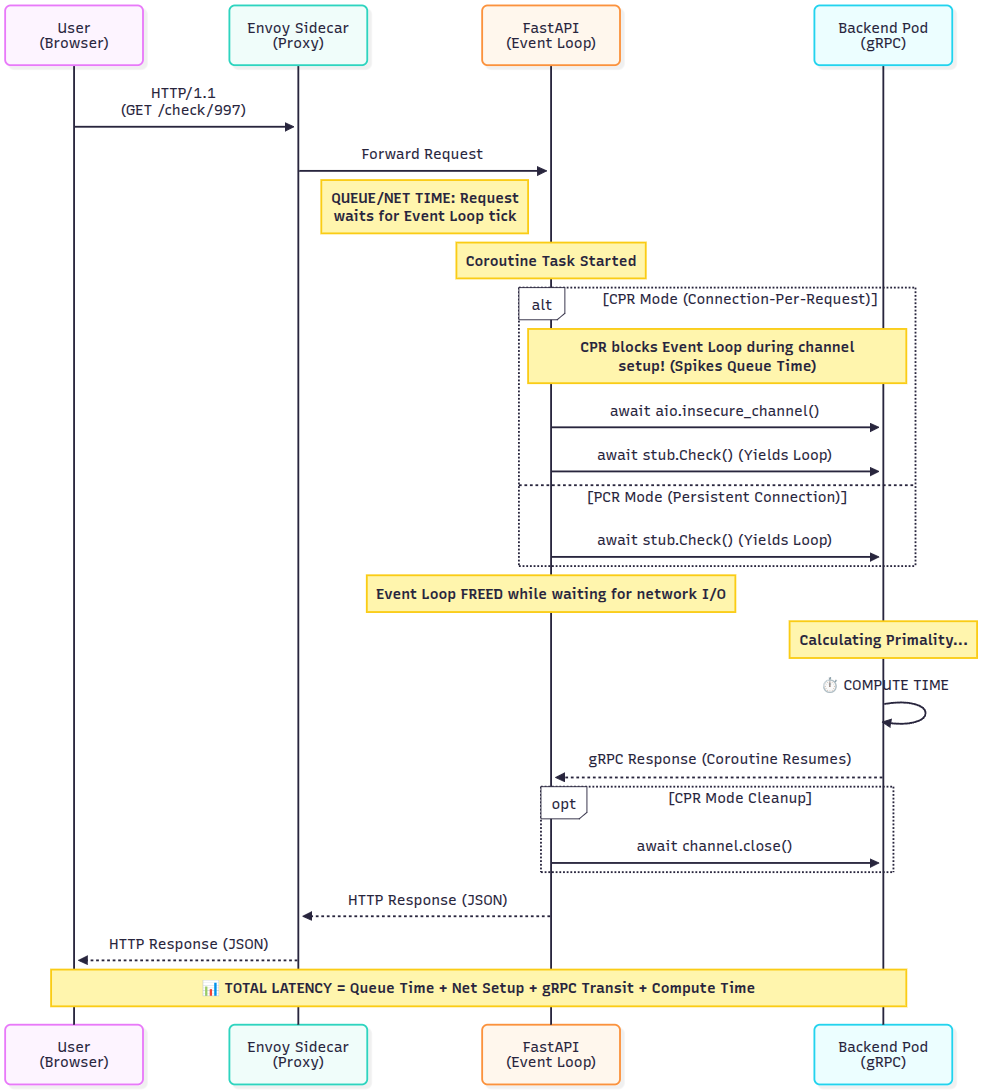
\includegraphics[width=\textwidth]{fig/seq-diagram-2-async.png}
		\vfill
		{\small (b)}
		\label{fig:async}
	\end{minipage}
	\caption{\textbf{Sequence diagrams comparing synchronous and asynchronous communication models in cloud-native applications across Connection-Per-Request (CPR) and Persistent Connection Reuse (PCR): (a) Synchronous CPR/PCR (Flask/Gunicorn); (b) Asynchronous CPR/PCR (Flask/Uvicorn).}}
	\label{fig:seq-model}
\end{figure*}



%%%%%%%%%%%%%%%%%%%%%%%%%%%%%%%%%%%%%%%%%%%%%%%%
\section{Related Work}
\label{sec:related-work}
%%%%%%%%%%%%%%%%%%%%%%%%%%%%%%%%%%%%%%%%%%%%%%%%

\subsection{Transport Protocols and Communication Overhead in Microservices}
Microservice architectures increasingly rely on high-performance Remote Procedure Call (RPC) frameworks, such as gRPC, to facilitate low-latency inter-service communication over HTTP/2.  Recent work reports that because gRPC uses HTTP/2 and Protocol Buffers, it can cut latency by about 30\% compared with REST for inter-service communication \cite{alzahrani2026scalable}. That kind of gain matters most when applications make many small synchronous calls, since serialization cost, request framing, and connection handling are paid repeatedly across a request path.   

While HTTP/2 multiplexing significantly reduces connection overhead compared to HTTP/1.1 REST interfaces, system performance remains highly sensitive to underlying transport-layer connection management. Existing benchmark studies demonstrate gRPC's superiority in execution time and resource utilization. Taha et al. point out that proactive performance prediction in microservice systems struggles with dynamic dependencies and multiplexing, especially because long and changing call chains add delay \cite{taha2024proactive}. When one service request triggers many downstream calls, queueing and contention on shared channels can make tail latency less predictable even if average latency stays low.

However, these studies predominantly assume persistent channel reuse (PCR) under steady-state workloads. Several aspects significantly influence and characterize the causes of increased tail latency and non-linear throughput degradation in cloud continuum environments—including ephemeral functions, rapid auto-scaling, connection-per-request (CPR) patterns, and connection churn—which frequently lead to the exhaustion of the OS TCP listen backlog. Biondani et al. found that gRPC performance degrades for large file transfers, and they attribute this to HTTP/2 transport behavior: over a 45 ms RTT path, the bandwidth-delay product interacts badly with HTTP/2 application-layer flow control, so throughput is throttled while senders wait for WINDOW\_UPDATE frames \cite{biondani2026mate}. This is important for inter-service design because it shows that HTTP/2 multiplexing helps most for many small concurrent exchanges, not for every traffic type.

\subsection{Control Loops and Traffic Management}
The use of autonomic computing paradigms based on the Monitor-Analyze-Plan-Execute with Knowledge (MAPE-K) feedback loop has become common practice to address performance issues in cloud-native settings \cite{armstrong2017towards}. Traditional implementations integrate autonomic managers into the service mesh or API gateway to handle dynamic autoscaling, circuit breaking, anomaly detection, and traffic activity \cite{carnevali2025compositional}. A recent article introduces machine learning and agentic control units to predict microservice anomalies \cite{toka2021machine}. Nevertheless, these approaches introduce non-negligible telemetry aggregation and decision latencies, making them less effective in responding to immediate network socket saturation \cite{qiu2020firm}. Furthermore, standard load-balancing techniques used in gRPC, such as client-side round-robin or fixed connection age limits, do not effectively address connection starvation problems when runtime conditions suddenly shift between CPR and PCR operational modes \cite{dautov2014utilising}.

\subsection{Positioning and Novel Contributions}
In contrast to existing static performance evaluations or resource-intensive AI-driven controller techniques, our approach introduces a lightweight, mathematically based autonomic controller tailored specifically for gRPC connection management. By clearly establishing the transition boundary between CPR and PCR paradigms through queueing dynamics, the proposed controller achieves sensing and actuation results within milliseconds. It reduces monitoring overhead in the baseline during normal operation, efficiently minimizes end-to-end tail latency ($p99$) across various load categories, and prevents throughput collapse during critical TCP backlog saturation.


%%%%%%%%%%%%%%%%%%%%%%%%%%%%%%%%%%%%%%%%%%%%%%%%%%%%%%%%%%%%%%%%%%%%%%%%%%%%%%%%%%
\section{Mathematical Modeling of gRPC Connection Management}
\label{sec:math-model}
%%%%%%%%%%%%%%%%%%%%%%%%%%%%%%%%%%%%%%%%%%%%%%%%%%%%%%%%%%%%%%%%%%%%%%%%%%%%%%%%%%

In order to comprehend the communication bottleneck, it is essential to break down the entire lifecycle of a request as it progresses through the API gateway. This analysis will help us identify the key stages and factors contributing to the bottleneck in the communication process. We model this environment by evaluating two distinct application gateway architectures: a synchronous model \cite{gunicorn} (e.g., Flask thread pools) and an asynchronous model \cite{uvicorn} (e.g., FastAPI event loops).

Let $T_{total}$ be the total end-to-end latency experienced by the client. We define $T_{total}$ as:
\begin{equation}
    T_{\text{total}} = T_{\text{http}} + W_{\text{queue}} + S_{\text{gateway}} + T_{\text{network}}
\end{equation}

Where:
\begin{description}
  \item[$T_{\text{http}}$]    : ingress HTTP processing time.
  \item[$W_{\text{queue}}$]   : queueing delay at the gateway's worker processes.
  \item[$S_{\text{gateway}}$] : service time required by the gateway to establish and execute the downstream gRPC call.
  \item[$T_{\text{network}}$] : physical network propagation delay and backend computation time (baseline constant $c \approx 3\ \text{ms}$).
\end{description}

The critical variable in our study is $S_{gateway}$. We model this variable under two distinct operational paradigms, representing the system state before and after the autonomic controller's intervention.

\subsection{Paradigm 1: Connection-Per-Request (CPR)}
\label{sec2.1}

In the Connection-Per-Request (CPR) anti-pattern, as shown in the CPR section of Fig. \ref{fig:seq-model}, the application gateway initializes a new gRPC channel for every incoming request. The service time $S_{cpr}$ is defined as:

\begin{equation}
    S_{cpr} = t_{tcp} + t_{http2} + t_{rpc} + t_{teardown}
\end{equation}

Where $t_{tcp}$ is the TCP 3-way handshake, $t_{http2}$ is the HTTP/2 SETTINGS frame negotiation, $t_{rpc}$ is the actual payload serialization/transmission, and $t_{teardown}$ is the TCP teardown (FIN/ACK). Because $t_{tcp}$ and $t_{http2}$ require multiple network round-trip times (RTTs) and significant CPU context switching, $S_{cpr} \gg t_{rpc}$.

In decentralized cloud-native architectures, the Client-side Proxy Routing (CPR) model dictates that the primary application container natively executes its own network routing and load balancing (e.g., utilizing native gRPC load balancing). This proxyless architecture minimizes intermediate network hops, optimizing baseline latency and reducing steady-state resource consumption. However, previous studies on proxyless service meshes demonstrate a critical vulnerability: the CPR model tightly couples the computational domain with the networking domain.

From a queueing theory perspective, the CPR model operates as a rigid $M/M/c$ queue. Under acute traffic surges, the network routing logic aggressively competes with the core application logic for limited CPU cycles and thread pools. When the system arrival rate approaches or exceeds the mathematical processing capacity ($\lambda \ge  \lambda_{sat}$), the application’s internal queue saturates rapidly, inevitably leading to dropped connections, unbounded tail latency, and catastrophic node failure.

\subsection{Paradigm 2: Persistent Channel Reuse (PCR)}
\label{sec2.2}

In the optimized Persistent Channel Reuse (PCR) pattern, as shown in the PCR sections of Fig. \ref{fig:seq-model} for both the synchronous and asynchronous gateway models, the architecture initializes a single, thread-safe gRPC channel during application startup. All incoming requests are multiplexed over this channel. The setup costs are amortized over millions of requests, approaching zero per request. Thus, the service time $S_{pcr}$ simplifies to:

\begin{equation}
    S_{pcr} = t_{rpc}
\end{equation}



The PCR model completely decouples the data plane from the application by offloading routing, load balancing, and telemetry to a dedicated, out-of-process sidecar proxy (Envoy). This structural shift is dynamically enacted by the autonomic controller when saturation is detected.

While conventional research often criticizes the PCR model for introducing a continuous ``service mesh tax'', permanent CPU, memory, and latency overheads during normal operations \cite{chen2025trade,zhang2026adaptive}, its architectural strength lies in robust queue management \cite{xiang2024cost}. In the PCR model, the injected sidecar acts as a highly optimized, asynchronous buffer \cite{santos2018analyzing}. It absorbs massive traffic spikes, manages connection backlogs, and applies intelligent backpressure, thereby protecting the underlying application container (whether running synchronous threads or an asynchronous event loop) from localized saturation.

\subsection{Queueing Theory and Non-Linear Saturation}
\label{sec2.3}

The catastrophic latency spikes observed in empirical testing cannot be explained by relying only on $S_{cpr}$ value. We apply an $M/M/c$ queueing model, where incoming requests arrive at rate $\lambda$ and are serviced by $c$ gateway computational resources at rate $\mu = 1/S_{gateway}$.

The utilization of the gateway system is $\rho = \frac{\lambda}{c \cdot \mu}$. According to Little's Law \cite{little2011or} and standard queueing theory, the average queuing delay $W_{queue}$ grows asymptotically as utilization $\rho \to 1$:

\begin{equation}
    W_{queue} \propto \frac{\rho}{1 - \rho}
\end{equation}

Because $S_{cpr}$ is significantly larger than $S_{pcr}$, the service rate $\mu_{cpr}$ is artificially low. Therefore, under the CPR paradigm, the system reaches critical utilization ($\rho \to 1$) at a much lower arrival rate $\lambda_{sat}$. When $\lambda$ exceeds this threshold, $W_{queue}$ approaches infinity, resulting in the massive latency spikes and connection timeouts observed in our baseline data.

To fully contextualize the performance disparity between the CPR and PCR approaches, it is necessary to distinguish the roles of the TCP session, the HTTP/2 stream, and application-layer channel management. A \textbf{TCP session} represents the underlying Layer-4 network socket, which incurs significant latency overhead to establish. An \textbf{HTTP/2 stream} is a lightweight, logical sequence of frames operating within that single TCP session; this is the native mechanism gRPC uses to multiplex thousands of concurrent requests over one connection.

The essential flaw of the CPR anti-pattern is that it actively circumvents this multiplexing capability. By instantiating and tearing down a gRPC channel within the local request handler, CPR forces the underlying HTTP/2 library to establish and destroy a unique TCP session for every single request, limiting multiplexing to a single stream per connection. Conversely, the PCR approach, enabled by the Envoy proxy, does not rebuild HTTP/2 features in the application layer. It is a structural design pattern that initializes a single, global TCP session, keeping the L4 connection persistent so that the native L7 HTTP/2 stream multiplexing functions as intended, seamlessly absorbing the load that causes the CPR model to fail.


\subsection{Framework-Specific Queueing Dynamics}
\label{sec2.4}

While the general queueing delay $W_{queue}$ reflects system-level saturation, the structural behavior under high concurrency diverges fundamentally depending on the application framework's concurrency model. We distinguish between the multi-threaded synchronous model and the single-threaded asynchronous event-loop model.

\subsubsection{Synchronous Thread-Pool Model ($M/M/c$)}
In the synchronous architecture (e.g., Flask \cite{gunicorn}), the system relies on a thread pool of $c$ parallel worker processes. Each worker handles a single connection sequentially. When a request initiates an un-multiplexed gRPC call under the CPR paradigm, the worker thread is blocked for the entire duration of $S_{cpr}$:

\begin{equation}
	T_{\text{blocked}} = t_{tcp} + t_{http2} + t_{rpc} + t_{teardown}
\end{equation}

When the arrival rate exceeds the aggregate thread processing capacity ($\lambda \ge c\mu_{cpr}$), all $c$ workers become simultaneously occupied in I/O waiting states. Subsequent requests are diverted to the OS-level TCP listen backlog. Once this backlog fills, incoming SYN packets are dropped, driving $W_{queue} \to \infty$ and causing immediate client-side connection timeouts.

\subsubsection{Asynchronous Event-Loop Model ($M/G/1-PS$)}
In contrast, the asynchronous architecture (e.g., FastAPI \cite{uvicorn}) executes over an event loop using non-blocking I/O primitives. Rather than modeling the system as $c$ discrete servers, it is more accurately characterized as an $M/G/1$ Processor Sharing ($PS$) queue, where a single execution thread distributes CPU time across $N_{\text{active}}$ concurrent tasks \cite{dalai2024novel}.

When an asynchronous request initiates a gRPC call, it registers an I/O callback and yields control back to the event loop during the latency window $t_{tcp} + t_{http2}$. The service time distribution $G$ is general rather than exponential due to asynchronous context switching. The average queueing delay under Processor Sharing is expressed as:

\begin{equation}
	W_{queue, PS} = \frac{\rho}{1 - \rho} \cdot S_{g}
\end{equation}

Because the event loop does not block physical threads during network negotiation, the effective capacity limit is decoupled from OS thread count and is instead constrained by event-loop tick duration and memory overhead. This enables the asynchronous gateway to hold thousands of partially completed connections in a pending state, delaying catastrophic packet drops far beyond the limits of the synchronous $M/M/c$ model.

\begin{algorithm}
	\caption{Autonomic Controller with Math-based Predictive \& SLA-Aware Dynamic Cutover}
	\label{alg:ctr}
	\begin{algorithmic}[1]
		\STATE \textbf{Inputs:} Poll interval $t_{poll}$, Minimum traffic threshold $\lambda_{min} = 10$, Latency SLA $L_{SLA} = 50$ ms
		\STATE \textbf{Initialize:} $cutover\_triggered \gets \text{False}$
		\WHILE{\textbf{true}}
		\STATE Sleep for $t_{poll}$ seconds
		\IF{$cutover\_triggered = \text{True}$}
		\STATE \textbf{continue} \COMMENT{Idling post-actuation}
		\ENDIF
		\vspace{2mm}
		\STATE \textit{Fetch Real-time Telemetry}
		\STATE $\lambda \gets \text{QueryPrometheus}(\text{Rate of Requests (RPS)})$
		\STATE $S_{cpr} \gets \text{QueryPrometheus}(\text{Average Service Time (s)})$
		\STATE $L_{p95} \gets \text{QueryPrometheus}(\text{App P95 Latency (ms)})$
		\STATE $n_{threads} \gets \text{QueryPrometheus}(\text{Active Threads})$
		
		\IF{$\lambda < \lambda_{min}$ \textbf{or} Telemetry is Null}
		\STATE \textbf{continue} \COMMENT{Wait for stable load}
		\ENDIF
		\vspace{2mm}
		\STATE \textit{Framework Auto-Detection \& Recalibration}
		\IF{$n_{threads} > 50$}
		\STATE $mode \gets \text{SYNC (Flask)}$
		%\STATE $c \gets n_{threads}$ \COMMENT{Capacity bounded by OS threads}
		%\STATE $\tau_{ratio} $
		\ELSE
		\STATE $mode \gets \text{ASYNC (FastAPI)}$
		%\STATE $c \gets n_{async\_event\_loop}$ \COMMENT{Estimated concurrent event loop tasks}
		%\STATE $\tau_{ratio} $
		\ENDIF
		\STATE $c \gets 1.0$ \COMMENT{Normalized parallel compute capacity}
		\STATE $\tau_{ratio} \gets 0.80$ \COMMENT{Target utilization threshold}
		\vspace{2mm}
		\STATE \textit{Calculate Queueing Saturation Threshold}
		\STATE $\lambda_{sat} \gets \frac{c}{S_{cpr}}$
		\STATE $\lambda_{trigger} \gets \lambda_{sat} \times \tau_{ratio}$
		\vspace{2mm}
		\STATE \textit{Dual-Condition Evaluation}
		\IF{$\lambda \geq \lambda_{trigger}$ \textbf{and} $L_{p95} \geq L_{SLA}$}
		\STATE $t_{start} \gets \text{CurrentTime}()$
		\STATE $\text{PatchDeployment}(\text{sidecar.istio.io/inject="true"})$
		\STATE $\text{WaitUntilReady}(\text{Deployment Replicas})$
		\STATE $\Delta t_{rollout} \gets \text{CurrentTime}() - t_{start}$
		\STATE $\text{LogActuationMetrics}(\Delta t_{rollout})$
		\STATE $cutover\_triggered \gets \text{True}$
		\ENDIF
		\ENDWHILE
	\end{algorithmic}
\end{algorithm}

The Algorithm \ref{alg:ctr} is represented to accommodate mathematical processes in this section. There are four main stages in the Algorithm \ref{alg:ctr}: fetch real-time telemetry, initialization, analysis, and action stages. The fetch real-time telemetry stages will continuously accept all metrics from Prometheus required in the following process. Further acquired metric descriptions will be explained in Section \ref{sec:auto-ctr}. The initialization stages will identify which gateway framework stacks (Flask or FastAPI) the requester (frontend) uses to load the request. In the analysis stages, all metrics are evaluated using the mathematical model as discussed in this section. The results of the analysis will trigger specific steps to switch the patch, determining whether the action will be activated or not on the envoy sidecar deployment for the frontend. If the patch is considered to be deployed, this process involves evaluating the deployment time, which calculates how much time is spent on the envoy sidecar patch implementation, ensuring that the deployment responds appropriately based on the analysis outcomes.


%%%%%%%%%%%%%%%%%%%%%%%%%%%%%%%%%%%%%%%%%%%%%%%%%%%%%%%%%%%%%%%%%%%%%%%
\section{Autonomic Controller Architecture}
\label{sec:auto-ctr}
%%%%%%%%%%%%%%%%%%%%%%%%%%%%%%%%%%%%%%%%%%%%%%%%%%%%%%%%%%%%%%%%%%%%%%%


\Figure[t!](topskip=0pt, botskip=0pt, midskip=0pt){fig/ctr-arc.png}
{ 
	\textbf{The autonomic controller architectures.}
	\label{fig:ctr-arc}
}



\subsection{Sensing Mechanism and Telemetry Acquisition}
\label{sec3.1}
The average service time, represented as $S_{cpr}$, serves as the fundamental calculation component in establishing the mathematical saturation limit of the autonomic controller. The controller relies on two complementary Prometheus telemetry metrics to accurately calculate the $S_{cpr}$ variable in a distributed environment (e.g., RKE cluster). The controller continuously evaluates both metrics for further analysis: \textit{grpc\_client\_roundtrip\_latency\_seconds\_sum} ($gRPC_{sum}$) and \textit{grpc\_client\_roundtrip\_latency\_seconds\_count} ($gRPC_{count}$).

On the one hand, the $gRPC_{sum}$ metric serves as a continuous accumulator, gradually increasing over time. It tracks the absolute total seconds spent processing and responding to incoming remote procedure calls within the application. On the other hand, the $gRPC_{count}$ metric acts as a straightforward digital counter, registering the exact volume of discrete requests that have successfully completed their lifecycle. 

To derive the real-time average service time for the control plane, the autonomic controller calculates the quotient of the rates of change of these two metrics over a sliding observation window. Mathematically, this relationship is expressed as the ratio of their respective variations over a specific time delta $\Delta t$:

\begin{equation}
	S_{cpr} = \frac{\Delta \textit{gRPC_{sum}}_{\Delta t}}{\Delta \textit{gRPC_{count}}_{\Delta t}}
\end{equation}

In the field of classical queuing theory, service time ($S$) is commonly used to represent the duration a physical or virtual server is actively engaged in a single unit of work. By utilizing native gRPC roundtrip metrics, the controller captures highly accurate, comprehensive processing measurements instead of isolated internal application timers. This duration inherently includes data serialization, framework event-loop overhead, and the core CPU execution required for the prime number calculations. These processes are ilustrated in the Fig. \ref{fig:ctr-arc}. 



\subsection{Calculation and Analysis}
\label{sec3.2}

\subsubsection{Predictive Mathematical Formulation}
To mathematically formalize the system's performance under increasing target rates, the system architecture is modeled as an $M/M/c$ queue. This assumes a Poisson arrival process for incoming requests with rate $\lambda$ (target rate), exponentially distributed service times with rate $\mu$ (where $\mu = 1 / S_{cpr}$), and $c$ parallel computing resources \cite{tijms2003first} \cite{Banerjee2023MTDDHJSMTA}. For the system to remain stable, utilization must remain below capacity ($\rho < 1$). As the target rate $\lambda$ increases toward the total service capacity $c\mu$, the system enters a state of high utilization. According to Erlang's C formula \cite{angus2001introduction}, the probability that an arriving request must wait in the queue ($P_Q$) is:

\begin{equation}
	P_Q = \frac{\frac{(c\rho)^c}{c!(1-\rho)}}{\sum_{n=0}^{c-1} \frac{(c\rho)^n}{n!} + \frac{(c\rho)^c}{c!(1-\rho)}}
\end{equation}

Consequently, the average expected wait time in the queue ($W_{queue}$) grows non-linearly:

\begin{equation}
	W_{queue} = \frac{P_Q}{c\mu(1-\rho)}
\end{equation}

As $\rho \to 1$, $W_{queue}$ approaches infinity. This mathematical phenomenon explains the severe spikes observed in empirical $p99$ tail latencies. Rather than waiting for system utilization to completely fail ($\rho \ge 1.0$), the controller continuously polls real-time telemetry to compute the empirical service time ($S_{cpr}$) and calculates the mathematical saturation limit ($\lambda_{sat}$) based on the application's theoretical concurrency ($c$):

\begin{equation}
	\lambda_{sat} = \frac{c}{S_{cpr}}
\end{equation}

To guarantee survivability, the controller defines a predictive intervention boundary ($\lambda_{trigger}$) using a configurable safety threshold ratio ($T_{ratio}$):

\begin{equation}
	\label{eq:trigger}
	\lambda_{trigger} = \lambda_{sat} \times T_{ratio}
\end{equation}

\subsubsection{SLA Evaluation and Bottleneck Verification} 
While the predictive trigger anticipates resource exhaustion using theoretical capacity as stated in equation \ref{eq:trigger}. However, it's crucial to verify the actual system degradation empirically to avoid any premature actuation. The controller achieves this through real-time Service Level Agreement (SLA) monitoring, specifically targeting the 95th percentile application latency ($L_{p95}$). To acquire this metric accurately, the control plane queries the \textit{grpc\_client\_roundtrip\_latency\_\break seconds\_bucket} histogram exposed directly by the application runtime. By calculating the 95th quantile from the rate of change across these distribution buckets over a one-minute sliding window, the system extracts a stabilized, real-time measurement of the tail latency. We rely on this internal gRPC telemetry rather than the external HTTP network timers. It strictly separates the application's true compute and event-loop processing delays from external network issues, such as TCP backlog saturation or service queuing in the service mesh.

Targeting the 95th percentile ensures the controller focuses on the degraded experience of the slowest requests while filtering out extreme, transient outliers (like the 99th percentile) that are often caused by routine garbage collection or minor operating system context switching. This observed $L_{p95}$ value is continuously evaluated against a rigid, configurable latency boundary ($L_{SLA}$, set to $35$ ms). Within the hybrid controller mode, this SLA evaluation acts as the definitive proof of exhaustion. The mathematical capacity limit ($\lambda_{trigger}$) flags that the system should be saturated based on average service times, but the $L_{p95}$ breach provides the empirical confirmation that the synchronous thread pool or asynchronous event loop has actually failed to process the current concurrent workload. By requiring this latency condition, the controller completely avoids false-positive mitigations during brief, harmless traffic bursts.



\subsection{Actuation and Dynamic Cutover}
\label{sec3.3}

The control framework directly solves architectural inelasticity by bridging the CPR and PCR states dynamically. To prevent false positives caused by transient network jitter, the controller implements a strict dual-condition actuation gate. The dynamic cutover is only authorized if the predictive mathematical limit is breached \textit{and} the empirical SLA is actively failing (exceeding the $35$ ms threshold). The final condition is defined as:

\begin{equation}
	\text{Trigger} \rightarrow \text{True} \quad \text{if} \quad (\lambda \ge \lambda_{trigger}) \land (L_{p95} > 35\text{ ms})
\end{equation}

Upon satisfying this dual-condition logic, the autonomic controller intervenes proactively. It initiates a dynamic patch to the frontend deployment within the Kubernetes control plane, applying the \textit{sidecar.istio.io/inject="true"} annotation. This action forces a rolling restart, attaching the Envoy proxy to the workload in real-time. By dynamically shifting from a low-overhead CPR topology to a highly resilient PCR topology exclusively when these two thresholds intersect, the controller caps the connection bottleneck and neutralizes exponential queuing delay before catastrophic SLA violations occur.



%%%%%%%%%%%%%%%%%%%%%%%%%%%%%%%%%%%%%%%%%%%%%%%%%%%%%%%%%%%%%%%%%%%%%%%
\section{Experimental Setup and Evaluation Scenario}
\label{sec:experiment}
%%%%%%%%%%%%%%%%%%%%%%%%%%%%%%%%%%%%%%%%%%%%%%%%%%%%%%%%%%%%%%%%%%%%%%%

To validate the proposed mathematical model and pinpoint accurately where latency overhead originates, we conducted controlled experiments in a containerized distributed setting. Our evaluation follows a strict component isolation strategy: we first measure end-to-end performance across the full system and then benchmark the backend service alone in order to distinguish computation time from communication-related delays. This was achieved by deploying a stateless, deterministic backend and enforcing Kubernetes Guaranteed QoS (matching CPU/memory requests to limits) to eliminate resource throttling and "noisy neighbor" interference. 

Our testbed uses a Python WSGI stacks (Flask/Gunicorn \cite{gunicorn} and FastAPI/Uvicorn \cite{uvicorn}) as a standard API gateway. We aim to check how gRPC connection churn impacts performance, not to compare frameworks. Synchronous threads are sensitive to blocking network inputs, highlighting queueing issues. Detailed infrastructure specifications are presented in Table \ref{tab:infra}.

%\begin{figure}
%	\centering
%	%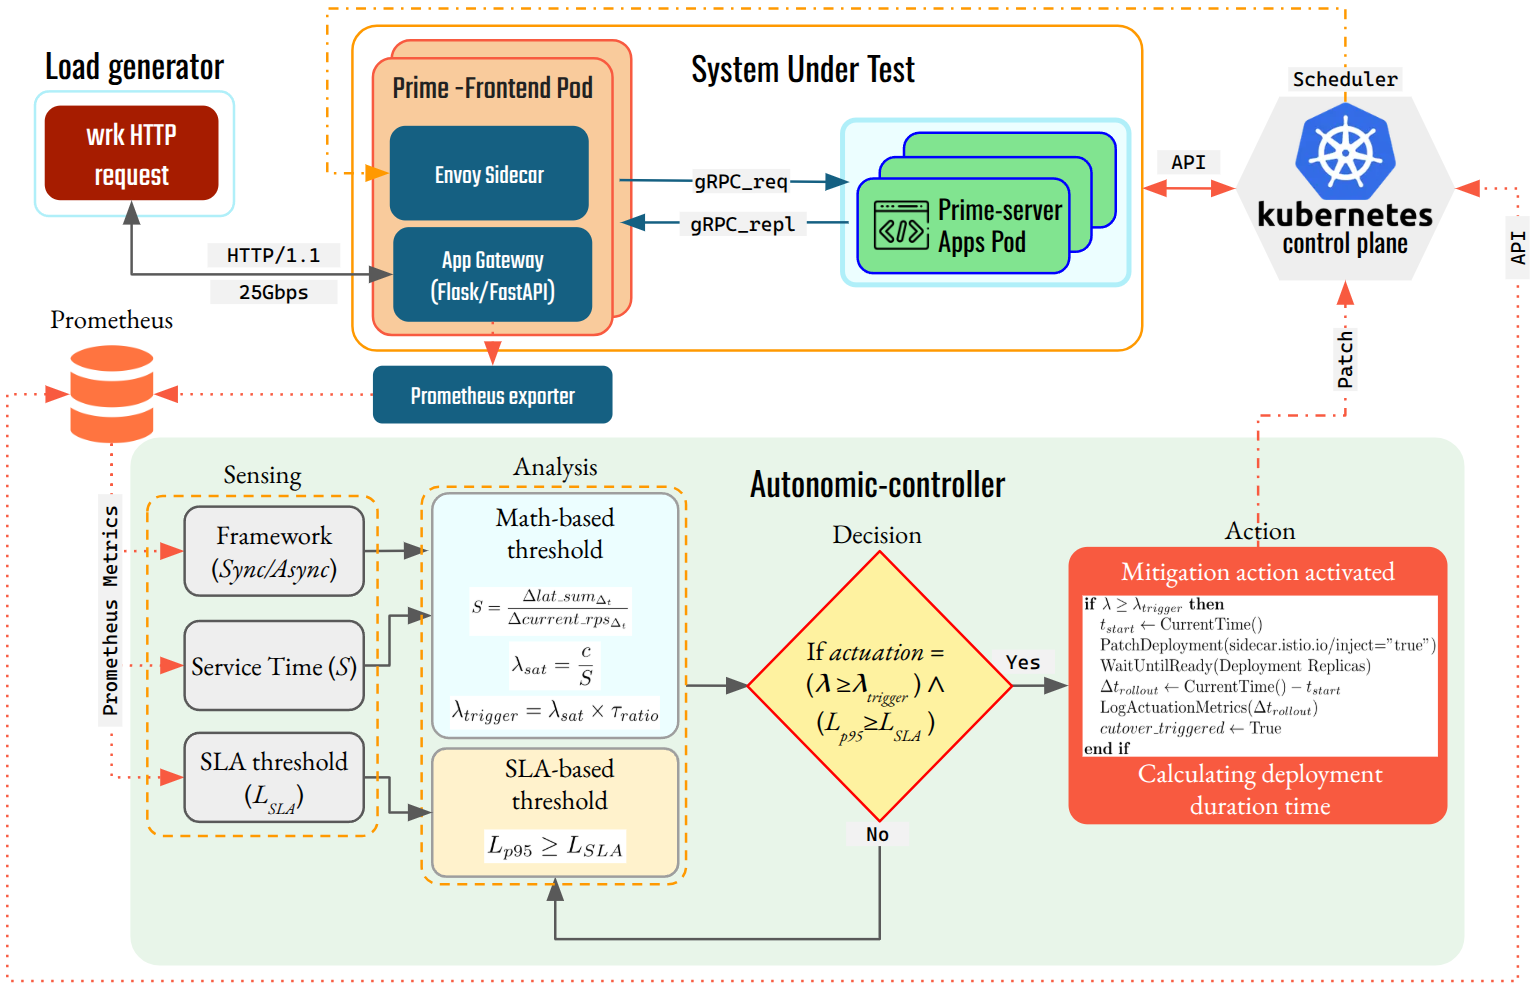
\includegraphics[width=\textwidth,height=0.25\textheight,keepaspectratio]{fig/ctr-arc.png} % or \linewidth
%	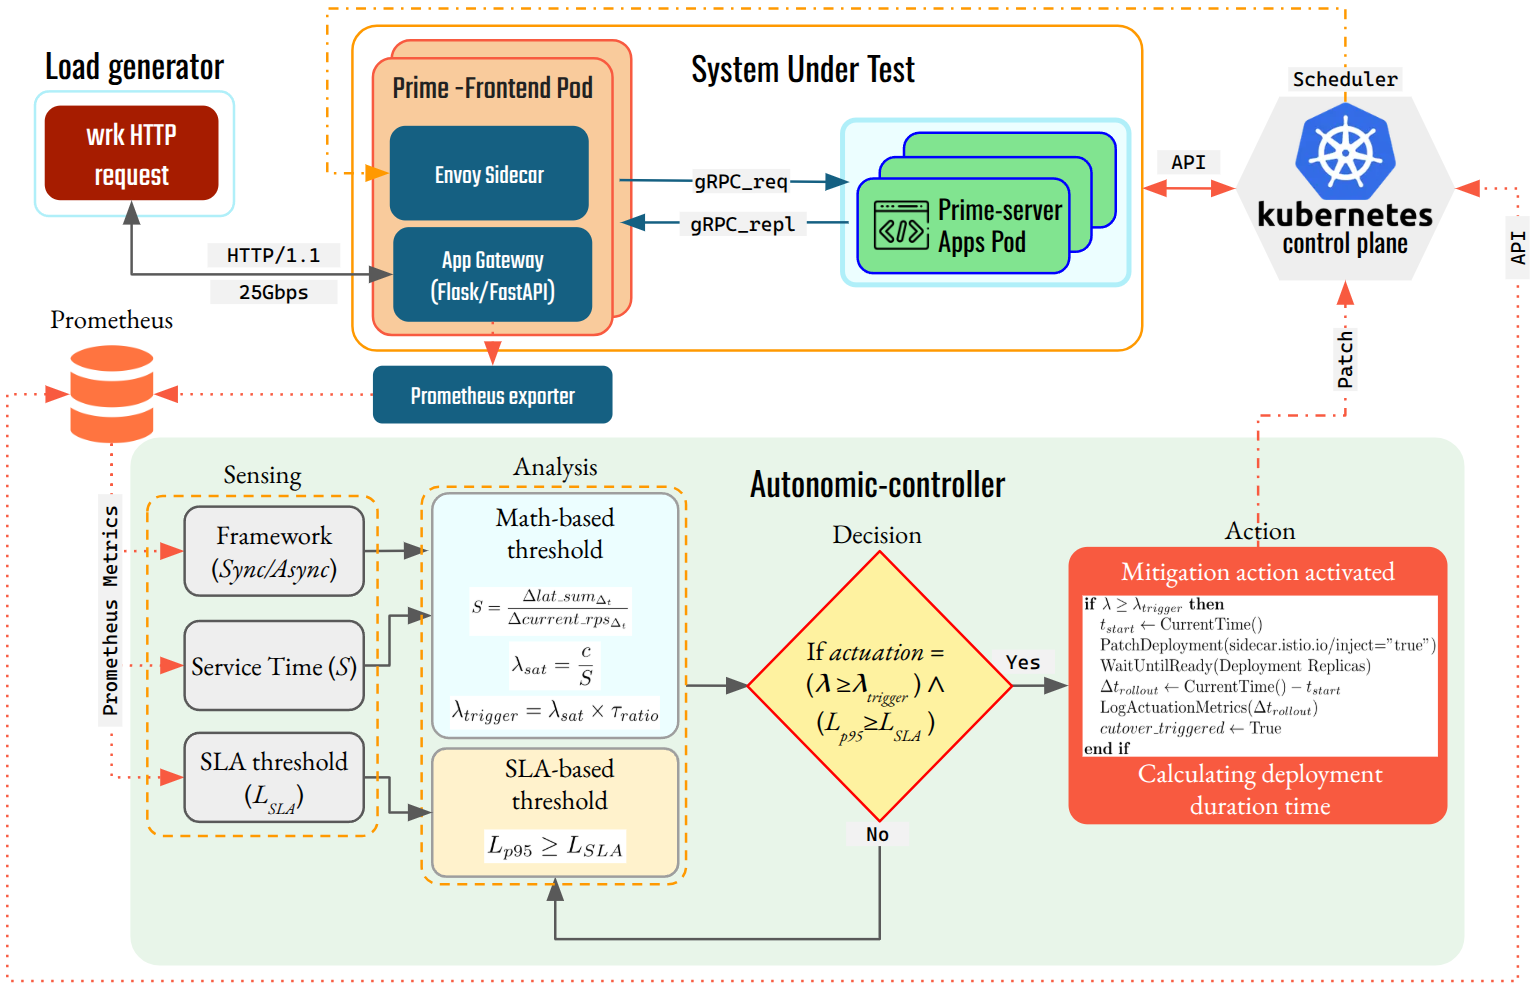
\includegraphics[width=0.45\textwidth]{fig/ctr-arc.png} % or \linewidth
%	\caption{\textbf{The proactive autonomic controller architectures.}}
%	\label{ctr-frame}
%\end{figure}

%\begin{figure}[t!]
%	\centering
%	\begin{minipage}{0.6\textwidth}
%		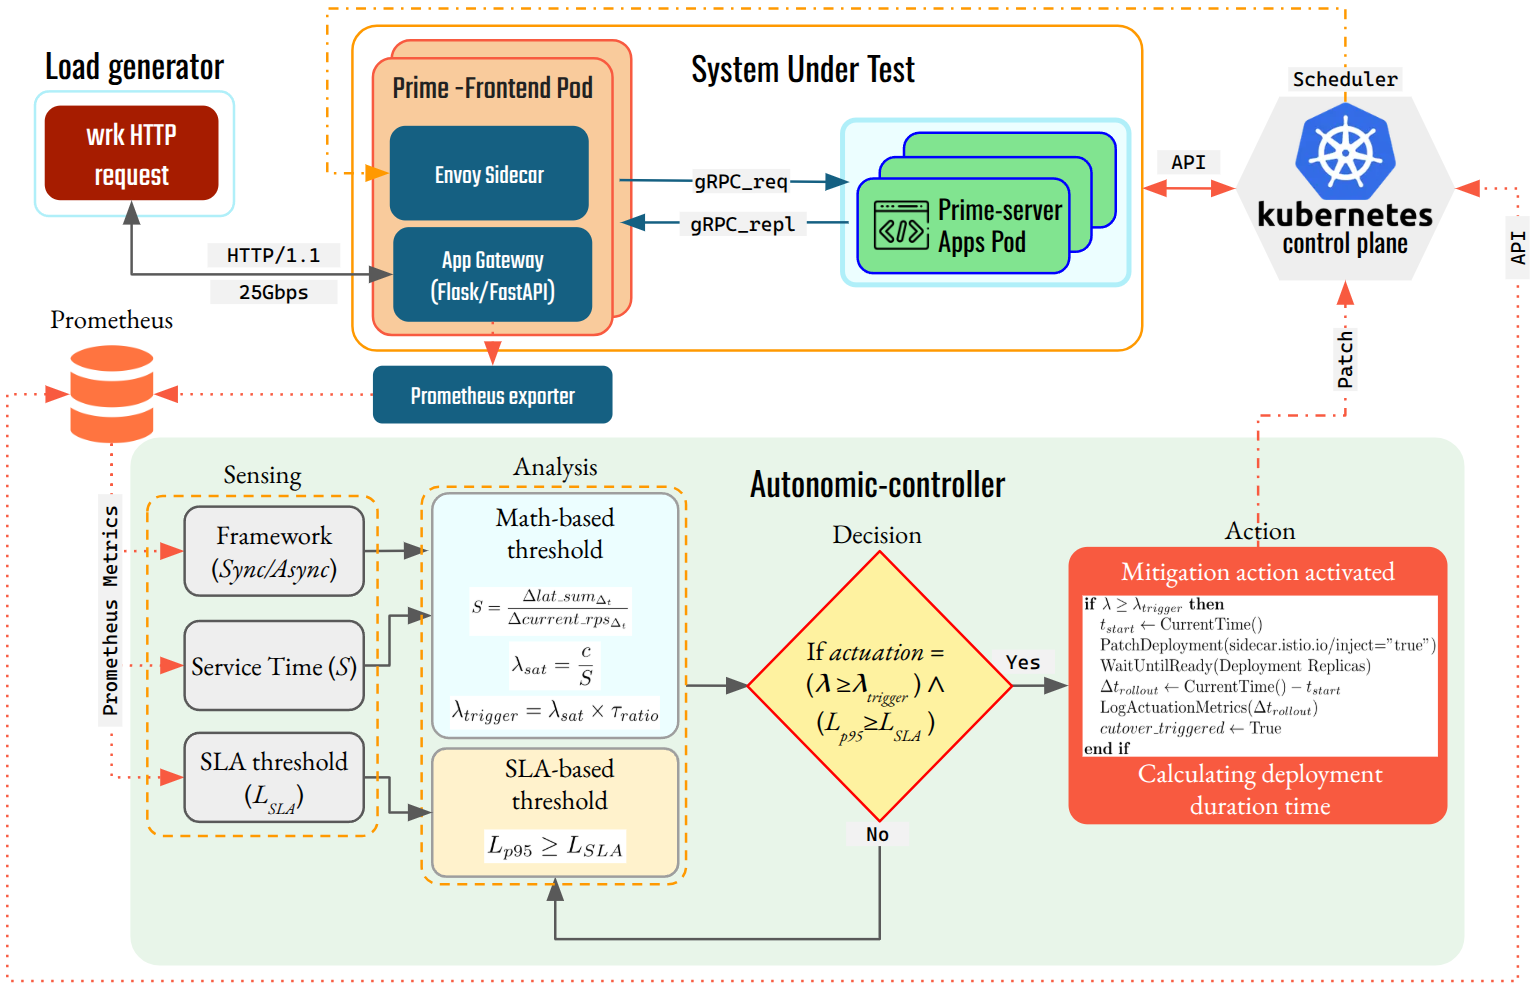
\includegraphics[width=\textwidth]{fig/ctr-arc.png}
%		\caption{\textbf{The proactive autonomic controller architectures.}}
%		\label{fig1}
%	\end{minipage}
%\end{figure}

\begin{table}[htbp]
	\centering
	\caption{\textbf{Infrastructure specification}}
	\label{tab:infra}
	\setlength{\tabcolsep}{3pt}
		\begin{tabular}{lcc}
			\hline
			\textbf{Components}& \textbf{Load generator (A)}& \textbf{SUT (B)}\\
			\hline
			CPU & Intel Xeon E-2274G (4 cores)& AMD EPYC 9655P (96 cores)\\
			Memory & 32GB & 194GB\\
			Storage & SSD 1TB & SSD 1TB\\
			Network & Mellanox MT27800 25Gb & Mellanox MT27710 25Gb\\
			OS & Ubuntu 22.04 LTS & Ubuntu 24.04 LTS\\
			K8s Cluster & RKE2 Control plane & RKE2 Worker  \\ 
			%\hline
			%\textbf{Gateway Overhead (PCR)} & $\sim 107.2$ ms & 97.5\% \\ 
			\hline
	\end{tabular}
\end{table}

\begin{figure}[t]
	\centering
	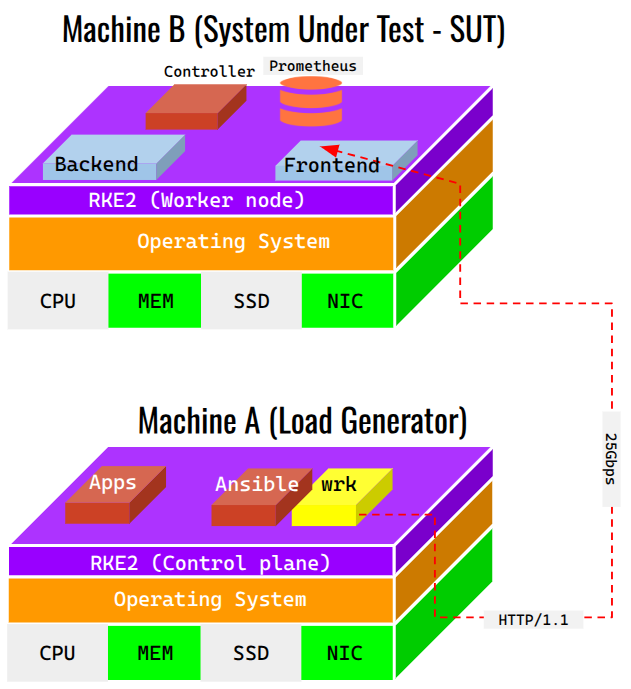
\includegraphics[width=\columnwidth,height=0.2\textheight,keepaspectratio]{fig/topology.png} % or \linewidth
	\caption{Kubernetes cluster environment.}
	\label{fig:rke-cls}
\end{figure}

\subsection{Experimental Environment and Architecture}
\label{sec4.1}

\begin{figure*}[t!]
	\centering
	
	\begin{minipage}{0.9\textwidth}
		\centering
		\vspace*{0pt}
		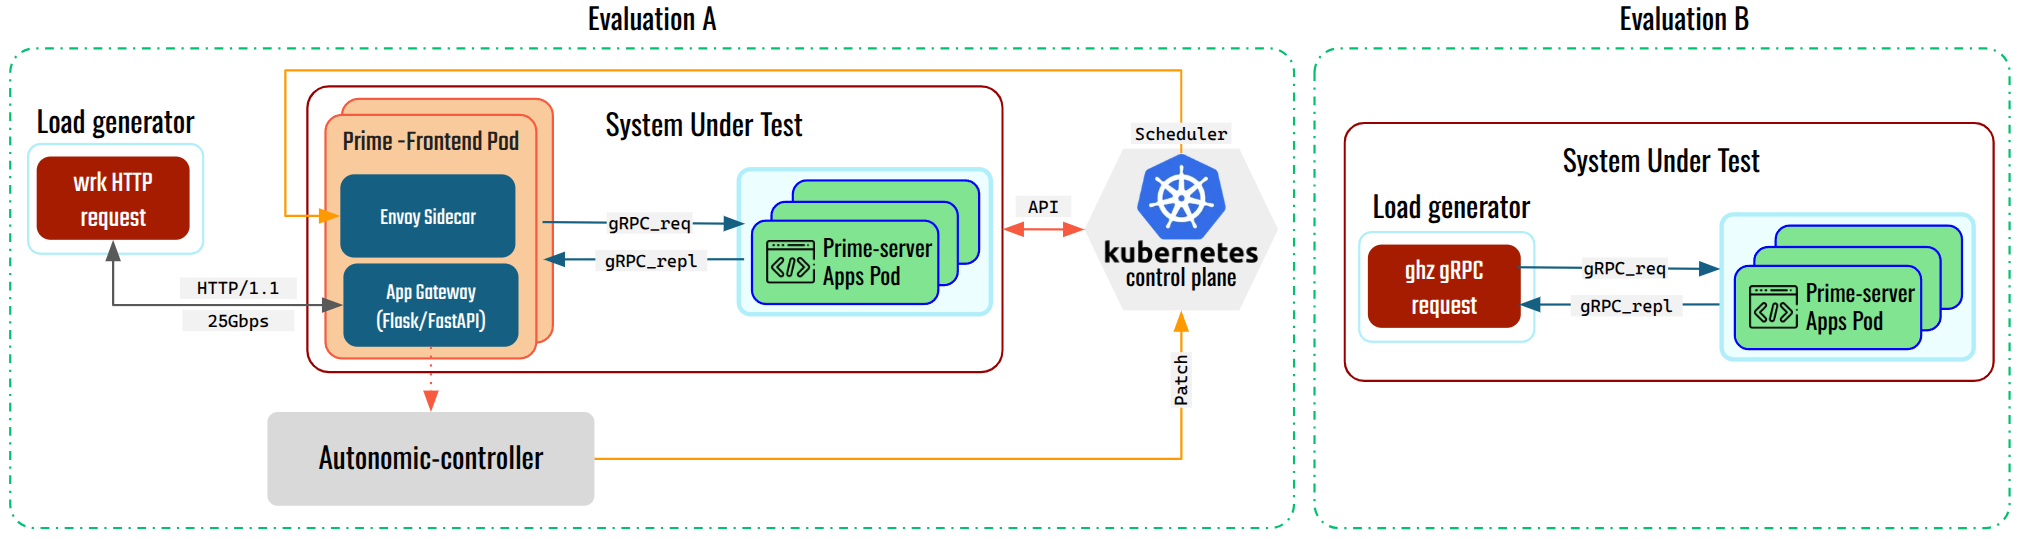
\includegraphics[scale=0.22]{fig/eval-stg.png}
		%\vspace*{4pt}
		%\centering{\small(a) Synchronous CPR/PCR (Flask/Gunicorn).}
		%\label{eval-stg}
	\end{minipage}
	%\vspace{10pt}
	\caption{\textbf{Evaluation scenario: (A) Comprehensive evaluations (end-to-end user experience); (B) Isolated backend service evaluation (compute time).}}
	\label{fig:eval}
\end{figure*}

The experiment was conducted on a Kubernetes cluster composed of multiple nodes, as shown in the Fig. \ref{fig:rke-cls}. In the Kubernetes cluster, machine A serves as the control plane, which is taints as a NoSchedule and NoExecute node. The end-to end load request will be executed from this node. To completely isolate the deployment application, machine B serves as the system under test (SUT) that consists of two main microservice components:

\begin{itemize}
    \item \textbf{gRPC Backend Service (prime-server)}: A high-performance Python application responsible for CPU-intensive prime number verification. To eliminate backend capacity as a confounding variable, this component was over-provisioned with 10 identical replica pods, deployed behind a Kubernetes NodePort Service.

    \item \textbf{API Gateway (prime-frontend)}: A Python Flask and FastAPI application running within Gunicorn and Uvicorn workers. This component acts as an HTTP/REST to gRPC proxy. It was strictly limited to 2 replica pods to intentionally force saturation and observe gateway-tier queuing dynamics under heavy load. 
\end{itemize}

\subsection{Component Isolation and Evaluation Scenario}
\label{4.2}


To precisely calculate the application-layer gateway overhead, we utilized two specialized, open-source load-testing tools (\textit{wrk2} \cite{wrk2} and \textit{ghz} \cite{ghz}), as shown in the Fig. \ref{fig:eval}:

\begin{itemize}
    \item \textbf{Unoptimized Gateway (CPR):} Simulates Algorithm~\ref{alg:ctr} ($mode = \text{CPR}$), forcing TCP/HTTP2 renegotiation for every incoming request.
    \item \textbf{Optimized Gateway (PCR):} Simulates Algorithm~\ref{alg:ctr} ($mode = \text{PCR}$), routing concurrent accesses through a single, globally initialized gRPC channel.
\end{itemize}


Both tools executed 30 iterations for each target throughput level (ranging from 100 to 1000 Requests Per Second, or RPS), sustaining the load for 60 seconds per iteration to allow queueing buffers to stabilize.

%\begin{figure}[t!]
%	\centering
%	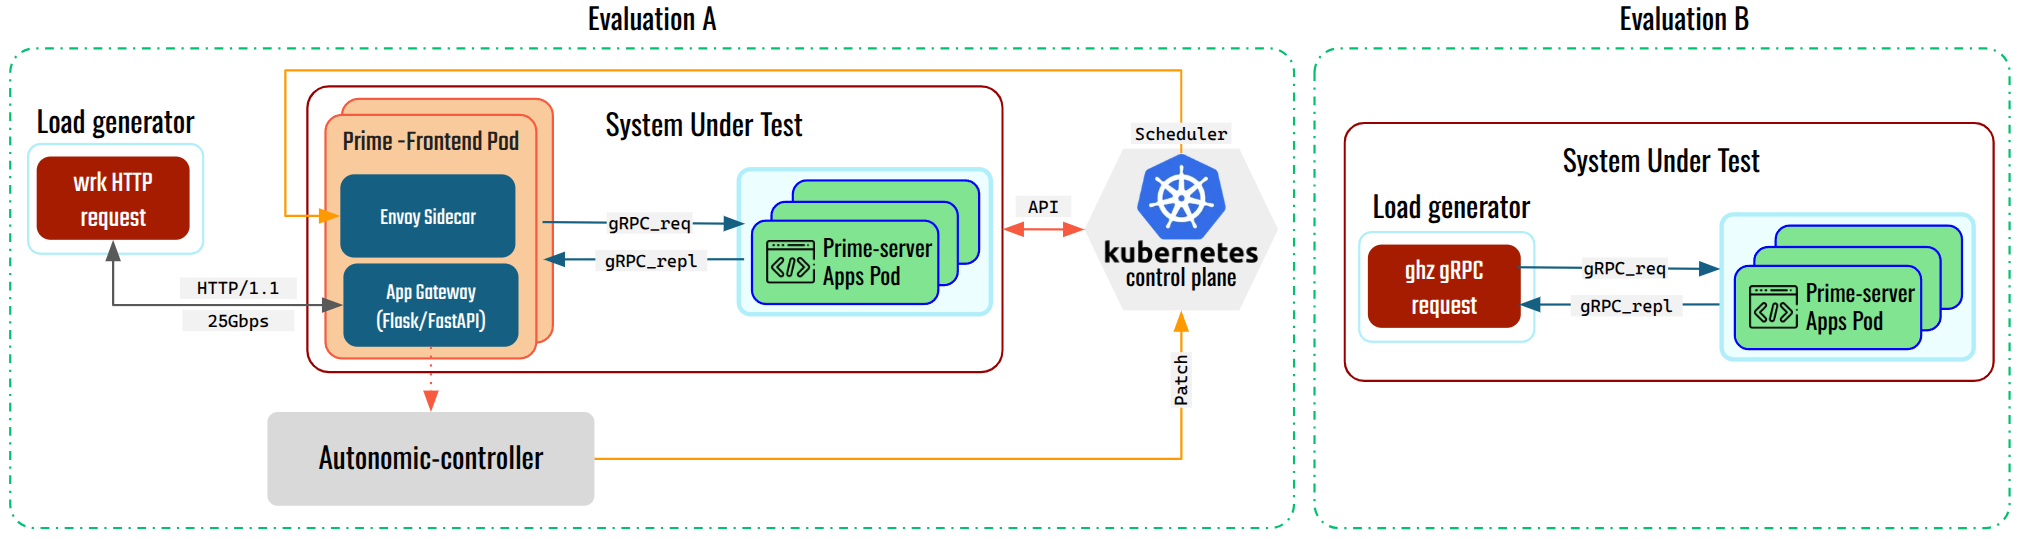
\includegraphics[width=\textheight,keepaspectratio]{fig/eval-stg.png} % or \linewidth
%	\caption{Evaluation scenario: (A) Comprehensive evaluations (end-to-end user experience); (B) Isolated backend service evaluation (compute time).}
%	\label{eval}
%\end{figure}

\begin{figure*}[t!]
	\centering
	\begin{minipage}{0.9\textwidth}
		\centering
		\vspace*{0pt}
		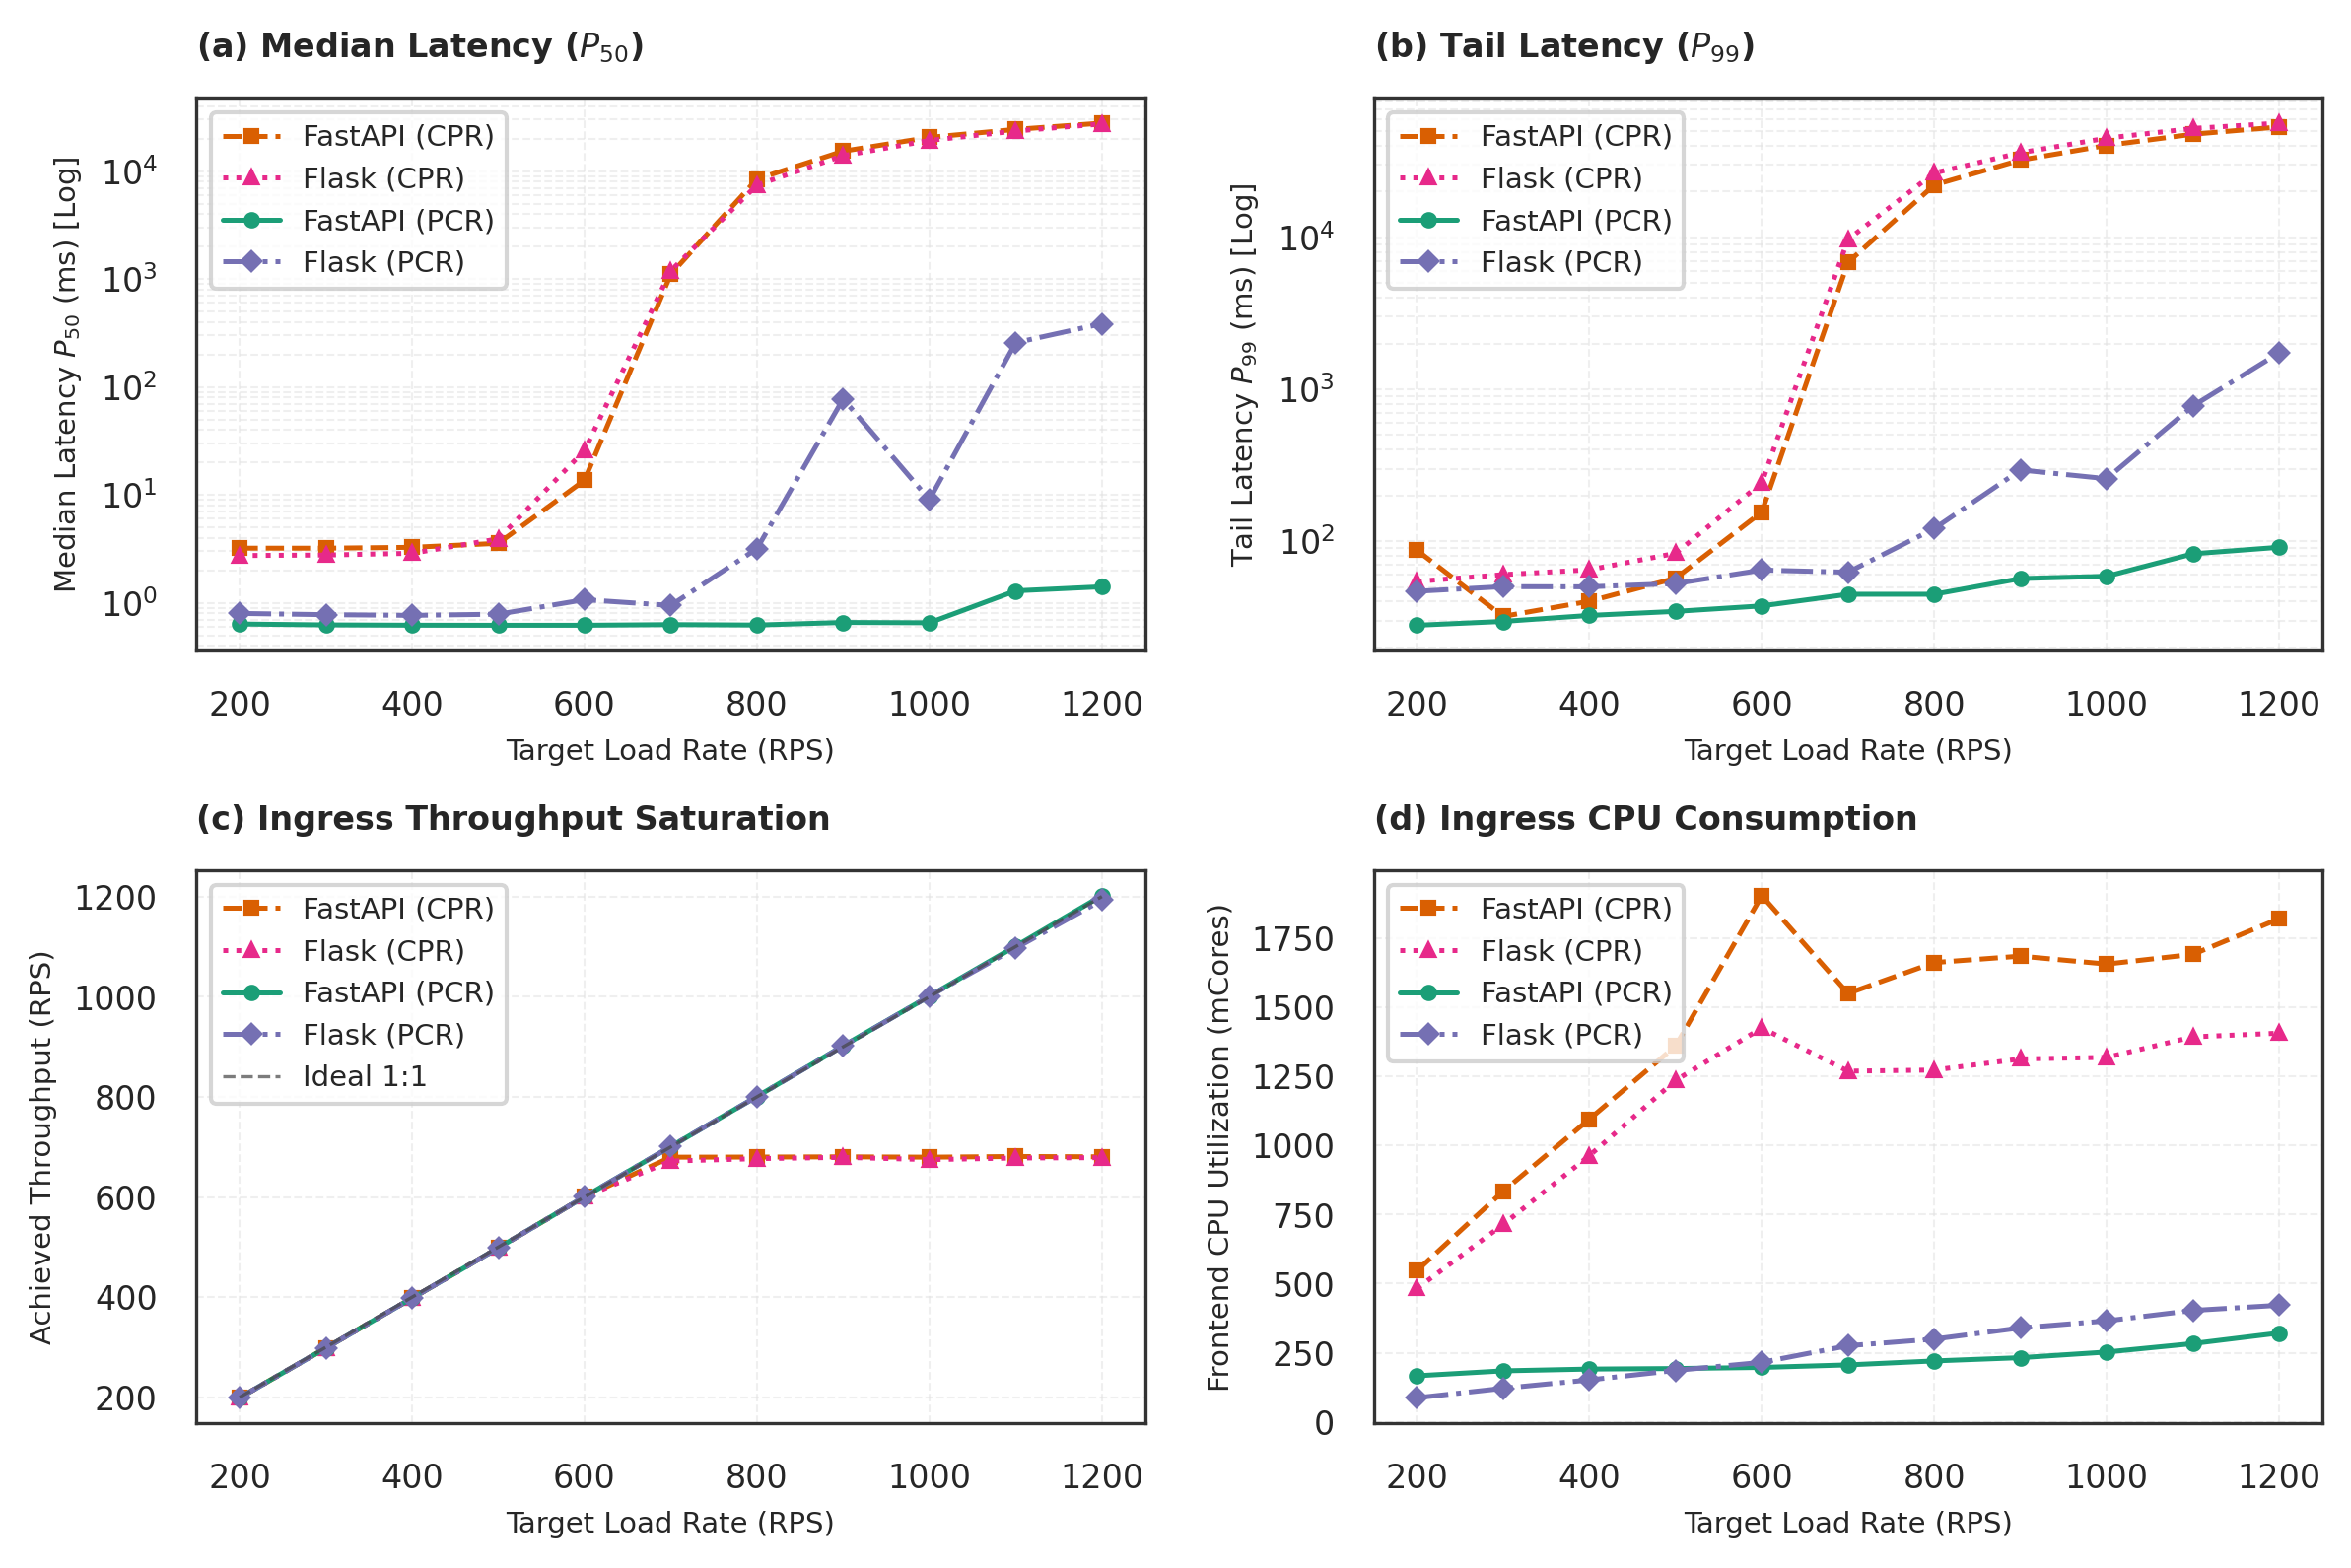
\includegraphics[scale=0.9]{fig/baseline_latency.png} % or \linewidth
	\end{minipage}
	\hfill
	\vspace*{5pt}
	\caption{Baseline performance evaluation of frontend communication gateway (Synchronous and Asynchronous method) within Connection Per Request (CPR) and Persistant Connections Reuse (PCR) model: (a) median latency ($p50$); (b) end-to-end latency ($p99$); (c) systems throughput; (d) resource utilization (CPU).}
	\label{baseline-perf}
\end{figure*}



%%%%%%%%%%%%%%%%%%%%%%%%%%%%%%%%%%%%%%%%%%%%%%%%%%%%%%%%%%%%%%%%%%%%%%%
\section{Results and Performance Analysis}
\label{sec:results}
%%%%%%%%%%%%%%%%%%%%%%%%%%%%%%%%%%%%%%%%%%%%%%%%%%%%%%%%%%%%%%%%%%%%%%%

The empirical results have successfully proven that the predicted Asymptotic latency degradation is caused by the $M/M/c$ queuing model in the Connection-Per-Request (CPR) paradigm and have clearly demonstrated the transformational impact of Persistent Channel Reuse (PCR). 


\subsection{Baseline: Backend gRPC Performance}
\label{sec5.1}

%\begin{figure}
%  \centering
%  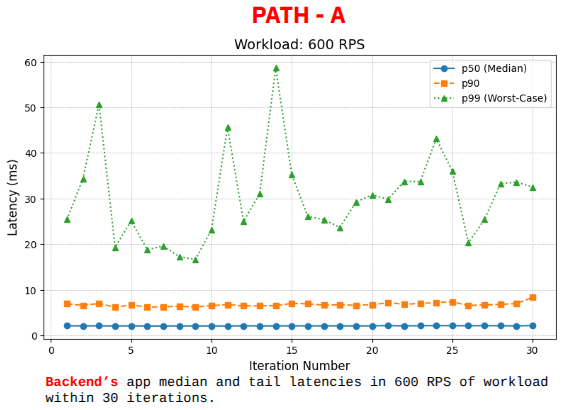
\includegraphics[width=\columnwidth,height=0.23\textheight,keepaspectratio]{fig/result2.png} % or \linewidth
%  \caption{gRPC backend latency evaluation using ghz benchmark tool.}
%  \label{fig4}
%\end{figure}

%\begin{figure}
%  \centering
%  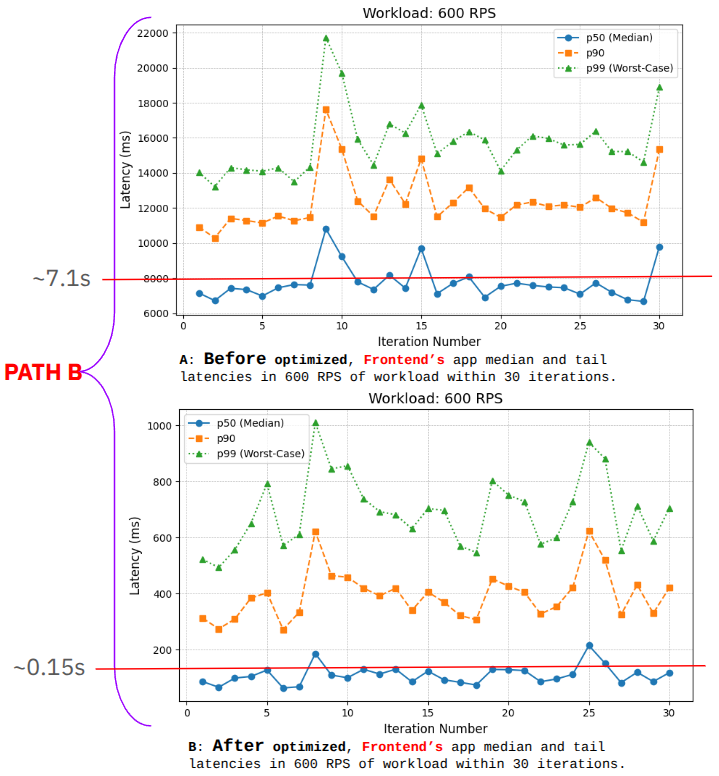
\includegraphics[width=\columnwidth,height=0.35\textheight,keepaspectratio]{fig/result1.png} % or \linewidth
%  \caption{End-to-end frontend latency evaluation using wrk2 as workload generator. (A) Connection-Per-Request paradigm - \textbf{Before} optimized, (B) Persistent Channel Reuse paradigm - \textbf{After} optimized}
%  \label{fig5}
%\end{figure}

The ghz test results established an exceptional and highly stable baseline. Across the entire load spectrum (100 to 1000 RPS), the 10 prime-server backend pods consistently delivered a median (p50) latency of $\sim 2.5 \text{ ms} \text{ to } 3.6 \text{ ms}$, with p90 latencies remaining firmly under 10 ms. 

This flat latency curve definitively proved that the backend architecture was not the system bottleneck, as shown in the Fig. \ref{fig4}. By having 10 backend pods, we mathematically guaranteed that the backend possessed vastly more computational capacity than the frontend could ever saturate. The computational capacity of the prime number verification logic was highly resilient, isolating the source of any overarching performance degradation to the gateway tier.

\textbf{Concurrency Configuration and Multiplexing:}
During empirical testing, both \textit{ghz} and \textit{wrk2} were configured to simulate high concurrency using a fixed pool of 50 simultaneous client connections across all target throughput levels ($\lambda$). It is critical to note how these concurrent accesses are handled internally by the optimized gateway. Under the PCR paradigm, the concurrent requests arriving at the gateway are not queued sequentially over the network; instead, the underlying gRPC framework maps these concurrent application-level accesses into discrete, parallel HTTP/2 streams over a \textit{single} shared TCP connection. This mechanism prevents connection exhaustion and directly validates our mathematical assumption that $S_{pcr}$ approaches pure RPC execution time without queuing at the network socket layer.




\subsection{Unoptimized System: The CPR Bottleneck}
\label{sec5.2}

Testing the end-to-end system utilizing the CPR paradigm revealed a catastrophic bottleneck, as shown in the Fig. \ref{fig5}-A (upper side). At a moderate load of 400 RPS, the system maintained a median latency of $\sim 400 \text{ ms}$. However, as throughput increased to 600 RPS, the system hit the critical utilization threshold ($\rho \to 1$).

Median latency exploded to $> 7,100 \text{ ms}$, and p99 latency spiked past $14,000 \text{ ms}$. This exponential degradation perfectly aligns with the queueing theory model where service time ($S_{cpr}$) is artificially inflated by excessive TCP/HTTP2 handshake overheads for every transaction. The gateway workers were entirely occupied managing network state rather than processing business logic.

\subsection{Optimized System: PCR Implementation}
\label{sec5.3}


\begin{figure*}[t!]
	\centering
	\begin{minipage}{1\textwidth}
		\centering
		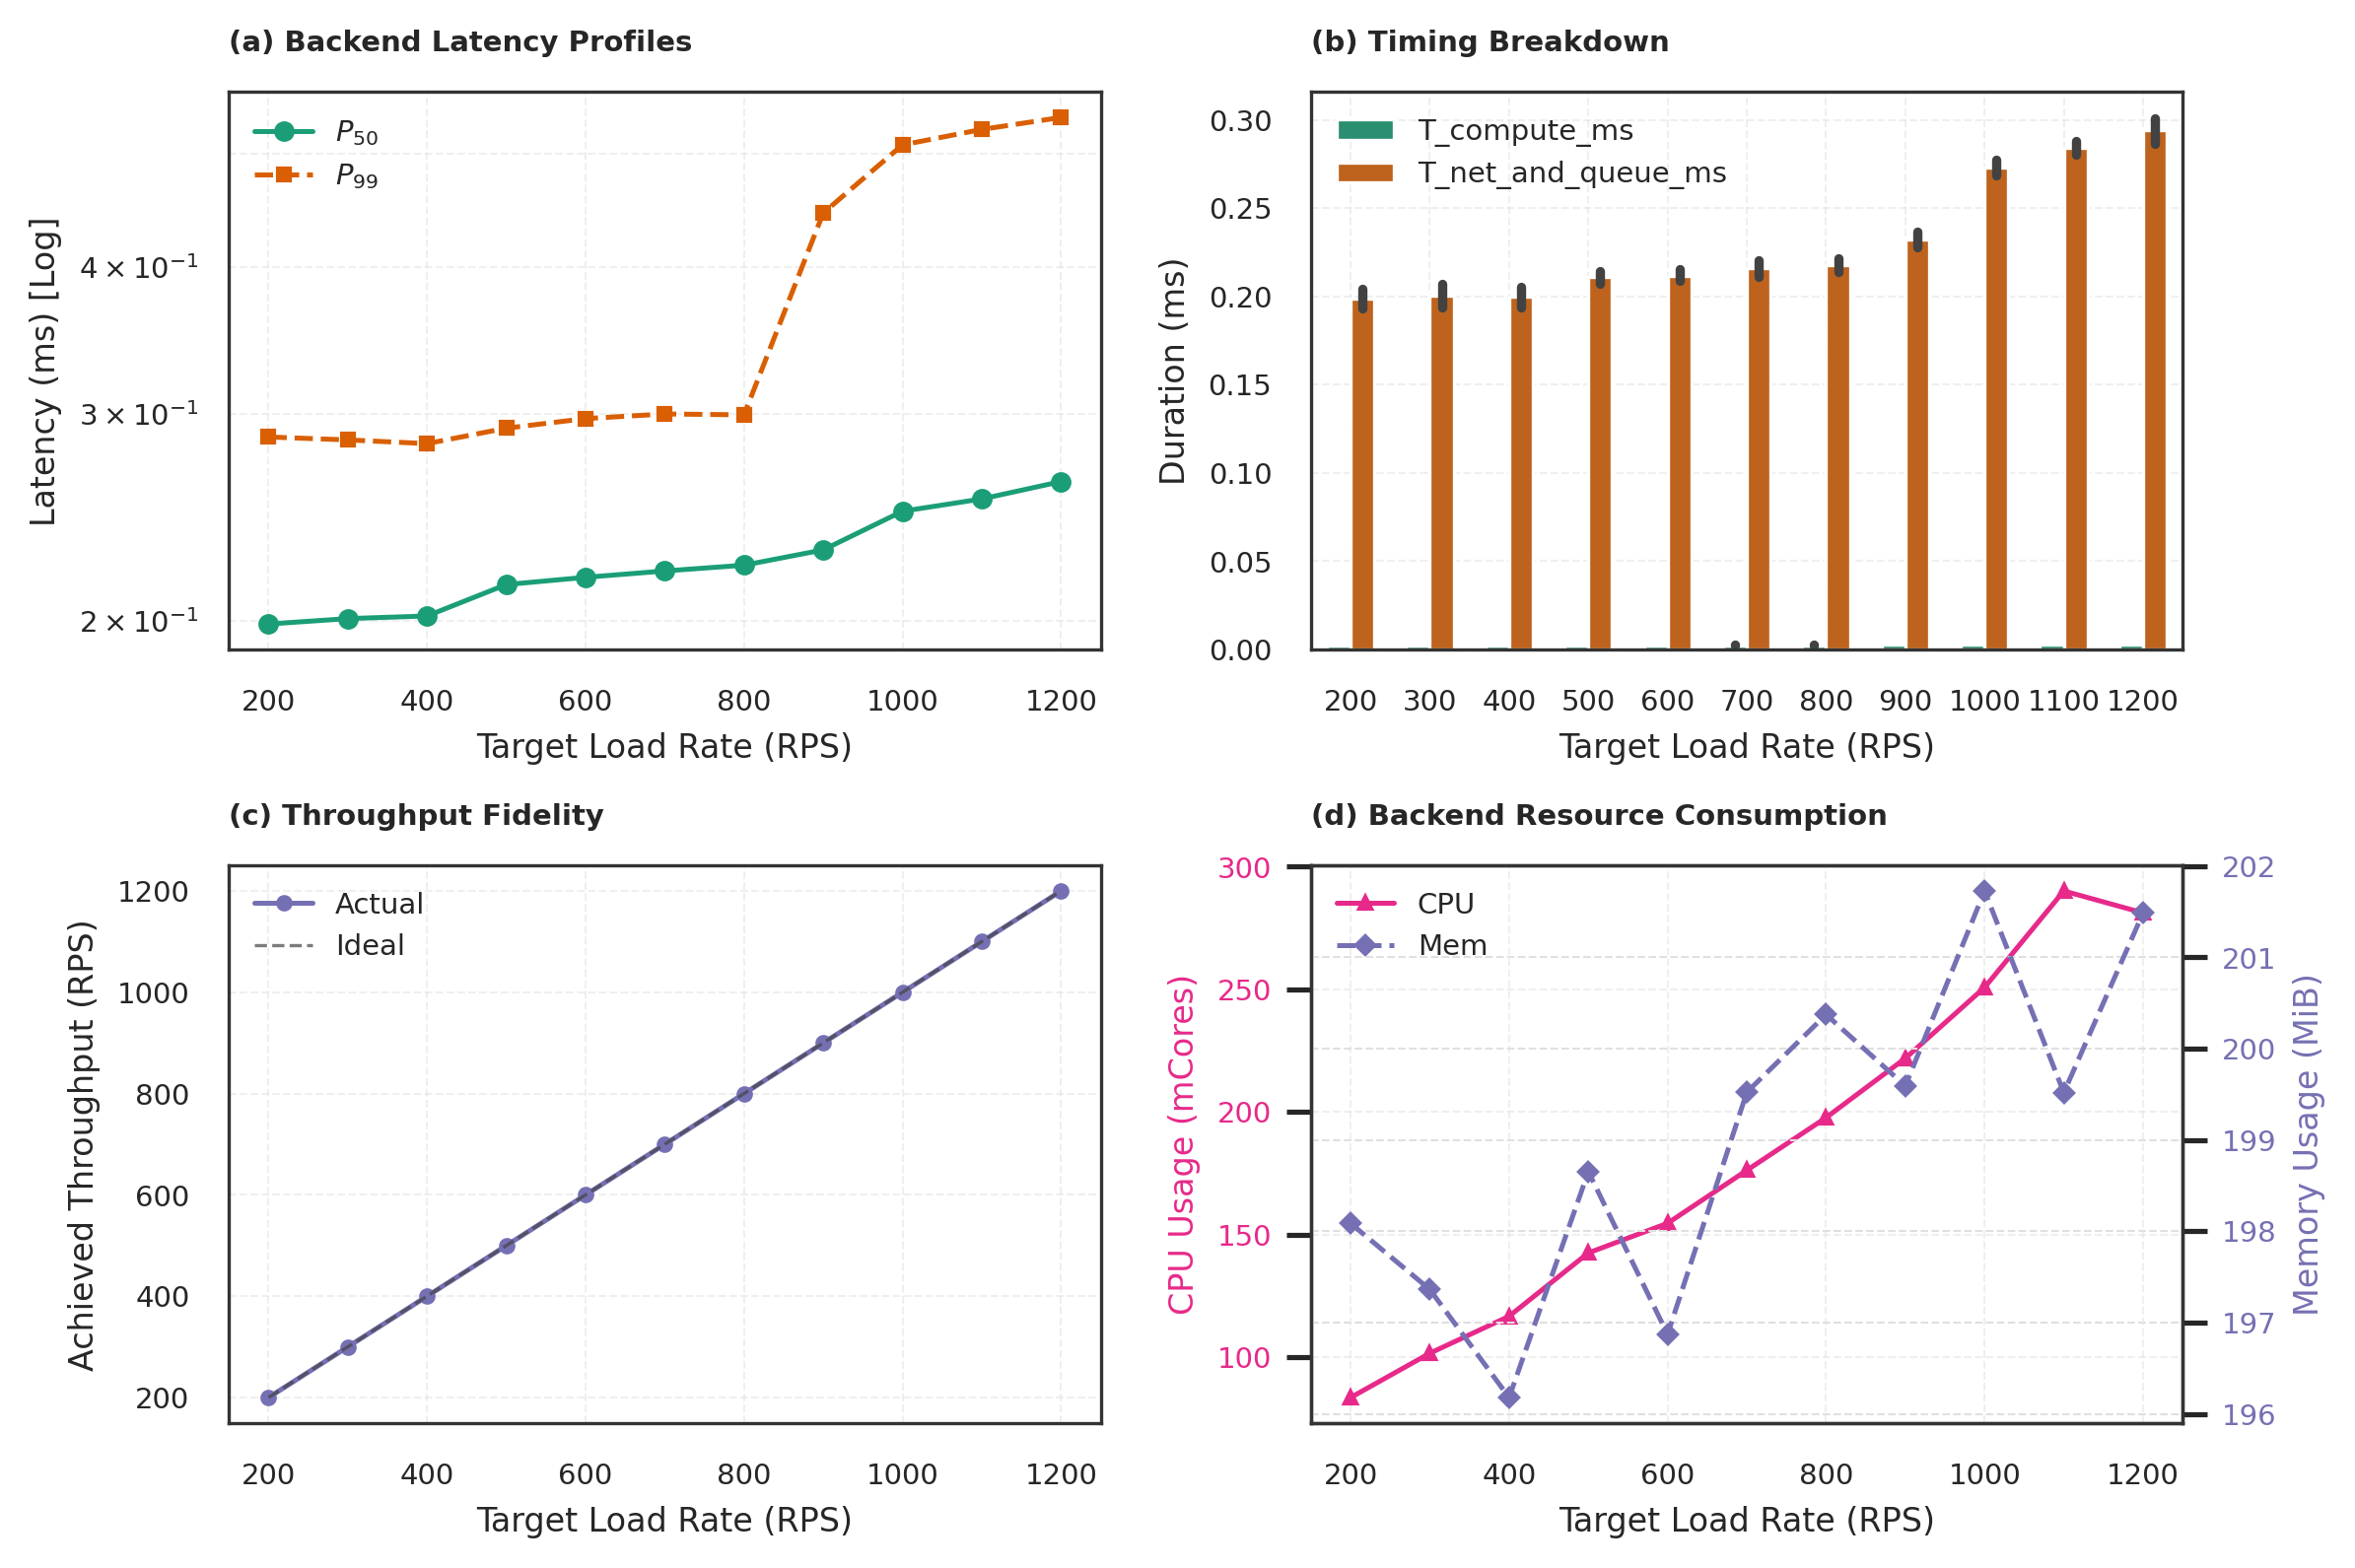
\includegraphics[scale=0.9]{fig/baseline_backend.png} % or \linewidth
		%\vspace{5pt}
	\end{minipage}
	
	\caption{Baseline performance evaluation of backend service that evaluate directly to the backend server using ghz tool with gRPC load request: (a) median and tail latency ($p50, p99$); (b) compute vs net and queue time latency ($t_{comp}, t_{net\_queue}$); (c) systems throughput; (d) resource utilization (CPU and Memory). These graphs are represent the result correspond to the evaluation scenario B on Fig. \ref{eval}.}
	\label{baseline-backend}
\end{figure*}

By deploying the algorithmic optimization detailed in Section \ref{sec3} (establishing a persistent, multiplexed gRPC channel at application startup - Algorithm \ref{alg1}), the performance profile of the system was qualitatively transformed.

At 600 RPS, the optimized system recorded a median latency of $\sim 150 \text{ ms}$, as shown in the Fig. \ref{fig5}-B (lower side). This represents a $\sim 97.9\%$ reduction in end-to-end latency compared to the CPR paradigm. Furthermore, the system successfully sustained loads up to 800 RPS before demonstrating signs of stress, effectively doubling the system's maximum throughput capacity without provisioning any additional infrastructure resources.

\subsection{Quantifying the Inherent Proxy Latency Gap}
\label{sec5.4}

By subtracting the baseline backend network latency ($T_{network}$) established via \textit{ghz} from the full end-to-end system latency ($T_{total}$) measured via \textit{wrk2}, we can isolate the underlying application-layer tax. We define this remaining overhead as the Inherent Proxy Latency Gap---the baseline latency strictly attributable to the framework's internal request handling, independent of network state management.

%\begin{table}[htbp]
%   \centering
%    \caption{\textbf{Comparative Latency Overhead at Optimal Saturation Point (400 RPS)}}
%   \label{table1}
%   \resizebox{\columnwidth}{!}{% <--- This scales the table to the column width
%    \begin{tabular}{lcc}
%    \toprule
%    \textbf{Component Level} & \textbf{Median Latency (p50)} & \textbf{Percentage of Total Latency} \\ \midrule
%    Backend Only (\textit{ghz}) & $\sim 2.8$ ms & 2.5\% \\
%    Full System (CPR, Before) & $\sim 400$ ms & 100\% \\
%    Full System (PCR, After) & \textbf{$\sim 110$ ms} & \textbf{100\%} \\ \midrule
%    \textbf{Gateway Overhead (PCR)} & \textbf{$\sim 107.2$ ms} & \textbf{97.5\%} \\ \bottomrule
%    \end{tabular}%
%    }
%\end{table}


\begin{table}[htbp]
	\centering
	\caption{\textbf{Baseline performance comparison across connection management strategies (CPR and PCR) and architectural paradigms (synchronous - Flask and asynchronous - FastAPI).}}
	\label{tab:ctr-tele}
	\setlength{\tabcolsep}{3pt}
	%\resizebox{\columnwidth}{!}{
	%\begin{tabular}{|p{110pt}|p{75pt}|p{100pt}|}
	\begin{tabular}{llllll}
		\hline
		% This is the header sets
		\textbf{Architecture}& \textbf{Load}& \textbf{CPU}& \textbf{Mem}& \textbf{T\_comp}& \textbf{T\_net}\\
		& \textbf{(RPS)}& \textbf{(m)}& \textbf{(Mi)}& \textbf{(ms)}& \textbf{(ms)}\\
			
		\hline
		
		% This is the column value
		Sync (Flask) CPR & 200  &  482.1 & 147.1 & 0.84 &    4.98 \\
		Sync (Flask) CPR & 600  & 1425.4 & 156.1 & 0.85 &   40.84 \\
		Sync (Flask) CPR & 1000 & 1318.9 & 174.4 & 0.86 & 20454.8 \\
		\hline
		
		Sync (Flask) PCR & 200  & 86.9  & 140.7 & 0.83 & 2.77 \\
		Sync (Flask) PCR & 600  & 215.1 & 141.1 & 0.87 & 6.83 \\
		Sync (Flask) PCR & 1000 & 365.2 & 141.8 & 0.87 & 36.31 \\
		\hline
		
		Async (FastAPI) CPR & 200  & 546.4  & 346.1 & 0.83 & 5.55 \\
		Async (FastAPI) CPR & 600  & 1904.2 & 355   & 0.82 & 25.14 \\
		Async (FastAPI) CPR & 1000 & 1656.6 & 367.7 & 0.83 & 20518.2 \\
		\hline
		
		Async (FastAPI) PCR & 200  & 166.4 & 344.9 & 0.86 & 1.29 \\
		Async (FastAPI) PCR & 600  & 196.7 & 345.4 & 0.84 & 3.02 \\
		Async (FastAPI) PCR & 1000 & 252.4 & 345.5 & 0.86 & 5.71 \\
		
		\hline
		% \vspace{5pt}
		\end{tabular}
\end{table}

As illustrated in Table~\ref{table1}, the results reveal a compelling paradox in the optimized PCR paradigm. Although the persistent channel implementation successfully averted queue saturation and achieved a 97\% reduction in total latency compared to the CPR baseline, a compositional analysis shows that the gateway tier still accounts for 97.5\% of the remaining end-to-end response time. 

This empirical gap directly connects our theoretical approach to the user experience. In our PCR model, the actual backend computational execution ($T_{network}$) requires only $\sim 2.8$ ms ($2.5\%$ of total time), while the remaining $107.2$ ms is consumed by the gateway. Critically, this gap encompasses not only the Python WSGI \cite{wsgi-pep} stack execution but also the protocol transcoding overhead—the computational cost of parsing incoming HTTP/1.1 JSON requests from \textit{wrk2} and serializing them into HTTP/2 Protobuf messages for the gRPC backend. 

This reveals a fundamental "Performance-Abstraction Paradox." While developers utilize API gateways to seamlessly bridge RESTful clients (HTTP/1.1) with high-performance microservices (gRPC), this protocol translation introduces a structural latency tax that dwarfs the business logic itself. Consequently, while our PCR optimization resolves protocol-level queue saturation, the absolute lower bound of system latency remains strictly dictated by the gateway's HTTP-to-gRPC transcoding efficiency.


\begin{figure*}[t!]
	\centering
	\begin{minipage}{0.45\textwidth}
		\centering
		\vspace*{0pt}
		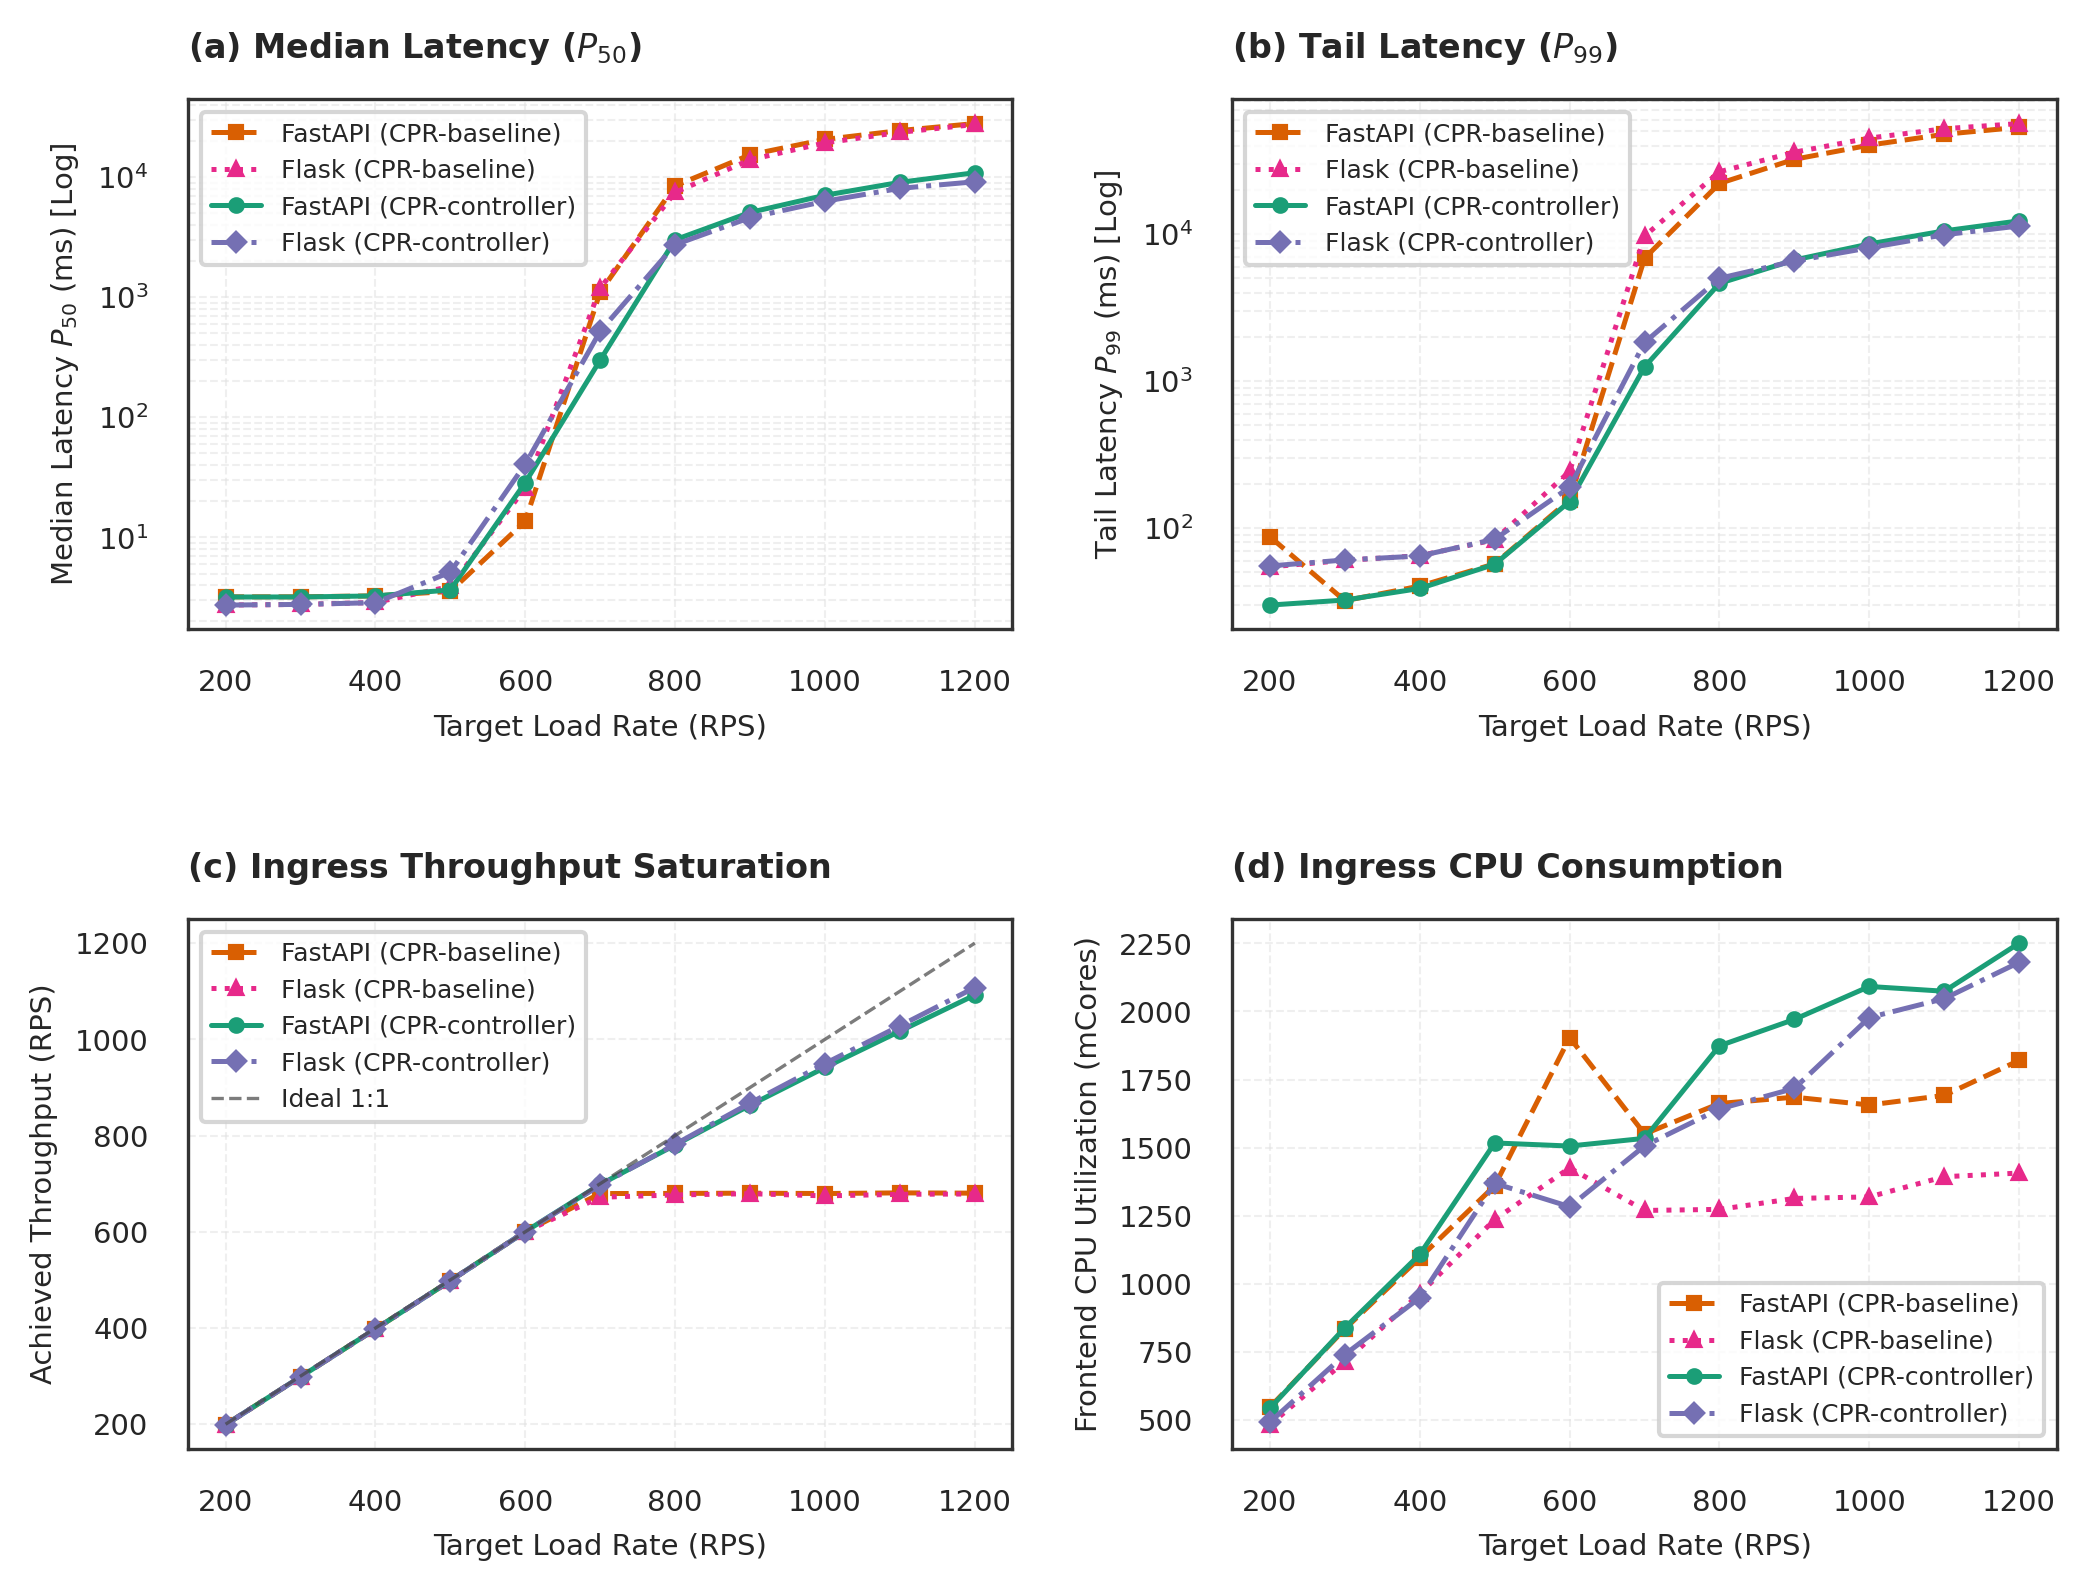
\includegraphics[scale=0.5]{fig/base_vs_ctr_cpr.png}
		\vspace*{4pt}
		\centering{\small(A)}
		%\label{eval-stg}
	\end{minipage}
	\hfill
	%\vspace{4pt}
	\begin{minipage}{0.48\textwidth}
		\centering
		\vspace*{0pt}
		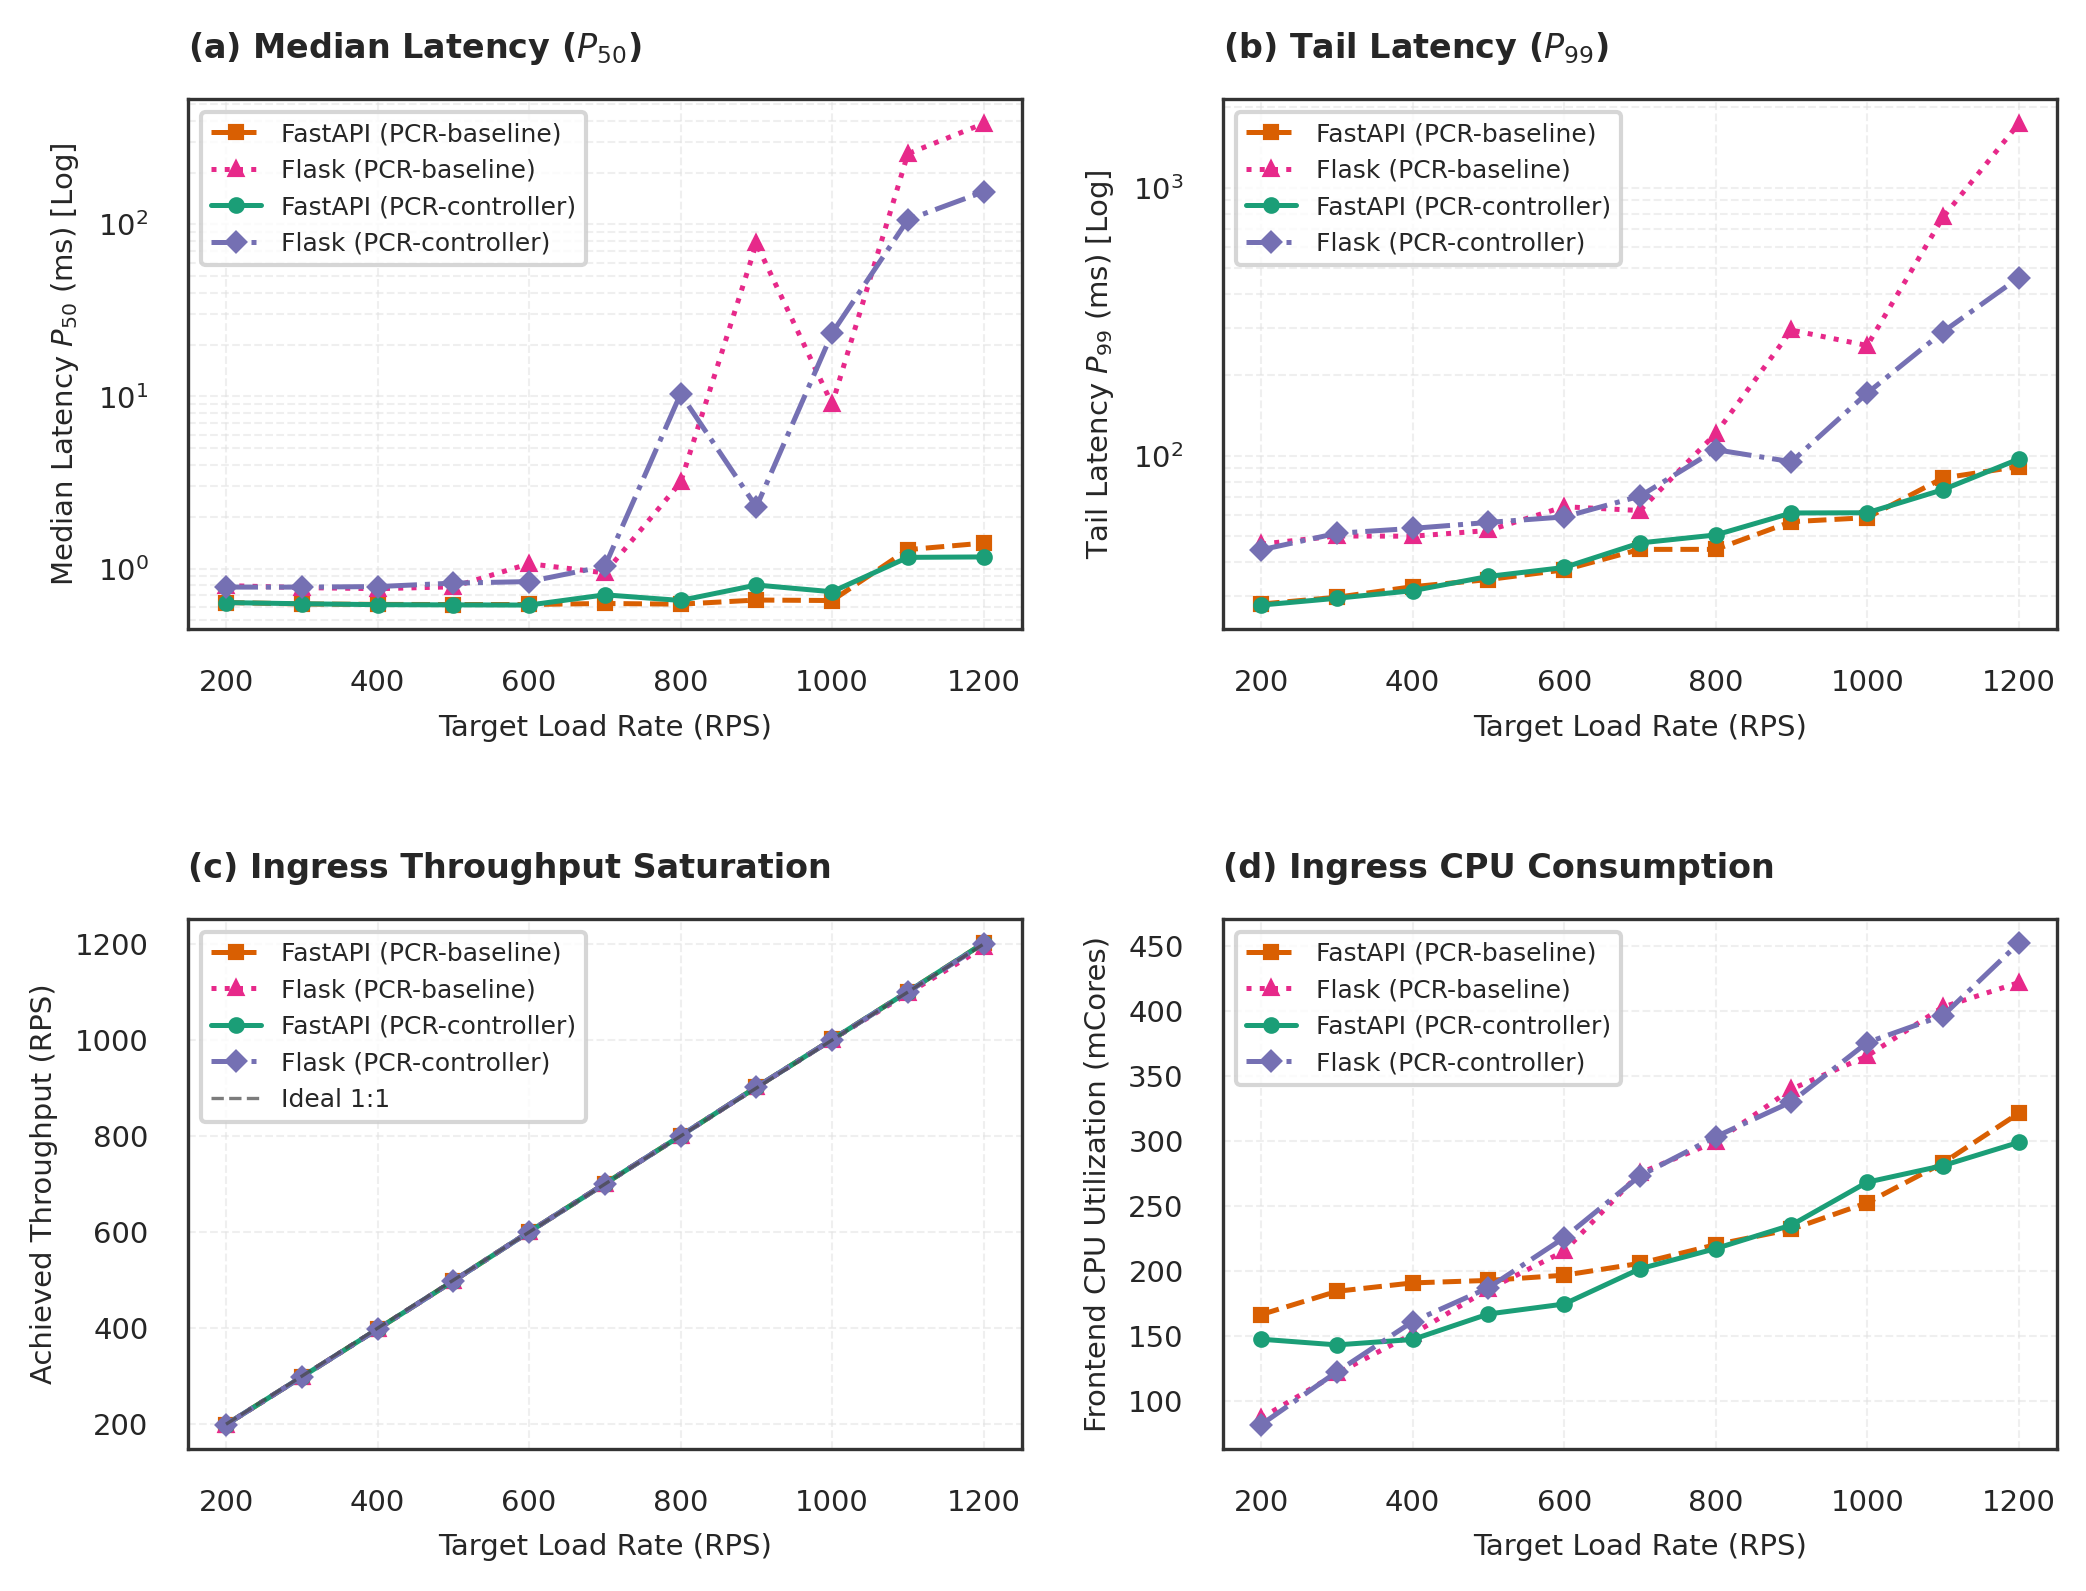
\includegraphics[scale=0.5]{fig/base_vs_ctr_pcr.png}
		\vspace*{4pt}
		\centering{\small(B)}
		%\label{eval-stg}
	\end{minipage}
	
	\caption{\textbf{Baseline vs controller performance evaluation of frontend apps both in Synchronous and Asyncronous framework gateway within: (A) Connection Per-Request (CPR); (B) Persistent Connection Reuse (PCR) mode.}}
	\label{base-vs-ctr}
\end{figure*}


\subsection{Empirical Validation of the Queueing Model}

\begin{figure*}[t!]
	\centering
	
	\begin{minipage}{1\textwidth}
		\centering
		\vspace*{0pt}
		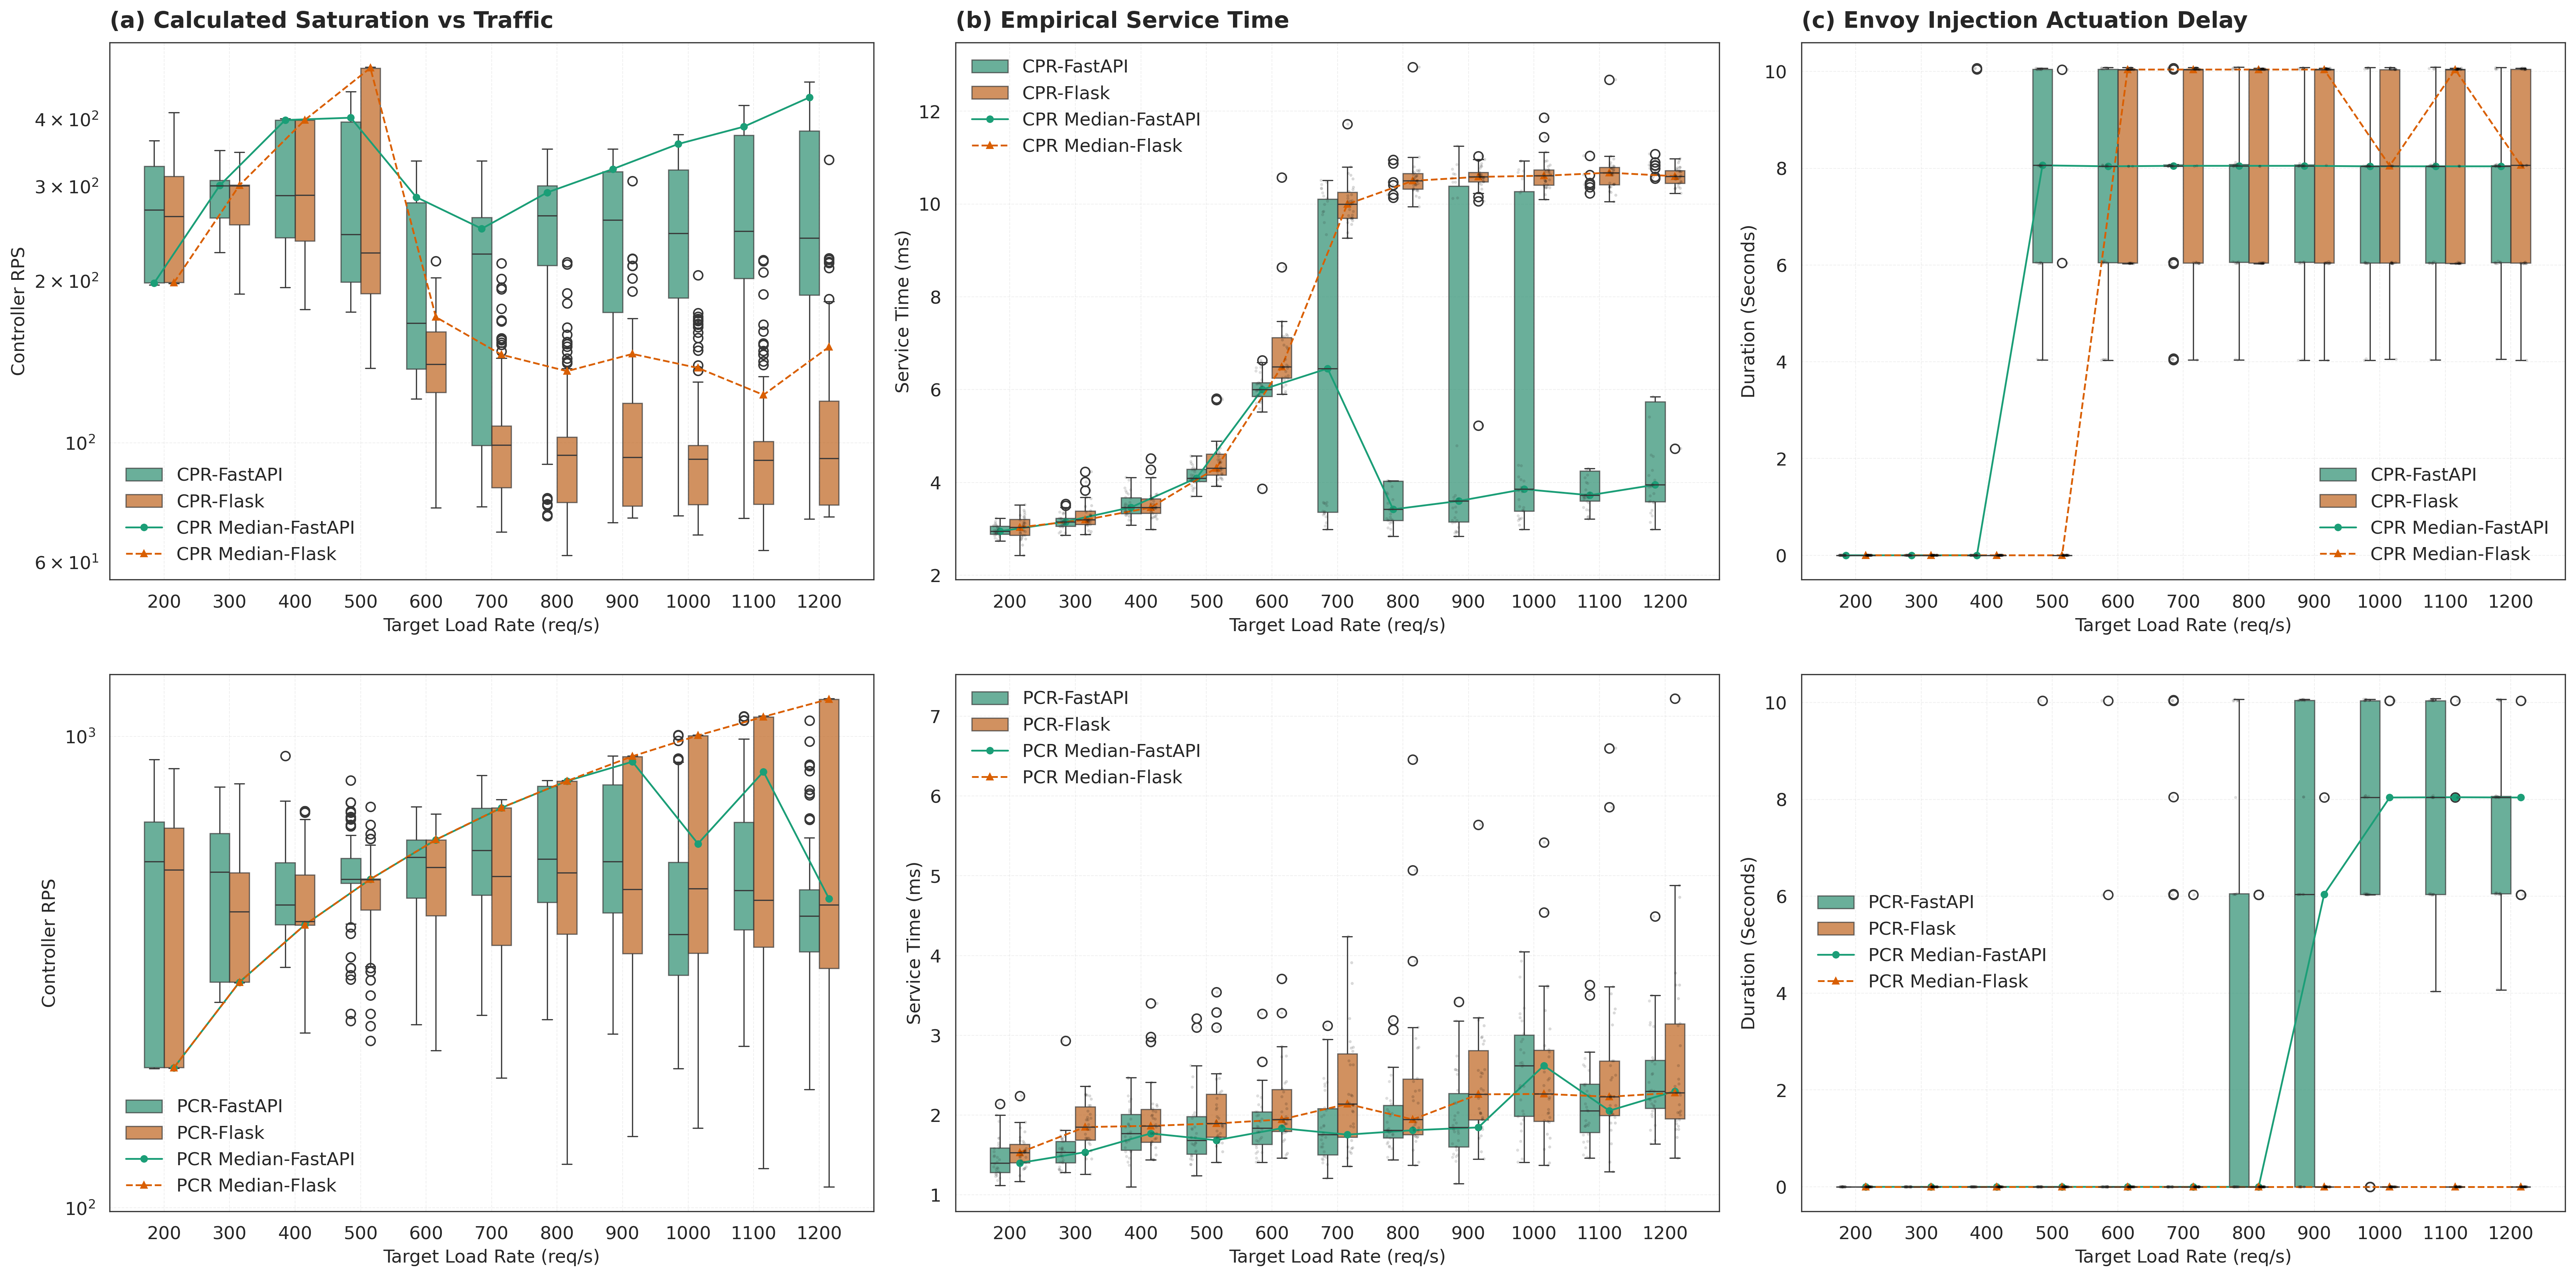
\includegraphics[scale=0.3]{fig/ctr-perf.png}
		%\vspace*{4pt}
		%\centering{\small(a) Synchronous CPR/PCR (Flask/Gunicorn).}
		%\label{eval-stg}
	\end{minipage}
	%\vspace{10pt}
	\caption{\textbf{Autonomic controller performance evaluation in asynchronous (FastAPI/Uvicorn) and synchronous (Flask/Gunicorn) mode. Connection Per Request (CPR) - upper row, Persistent Connection Reuse (PCR) - lower row : (a) Calculated saturation point ($\lambda_{sat}$); (b) service time ($S$); (c) Actuation time when envoy deployed to frontend pods.}}
	\label{eval-ctr}
\end{figure*}


To rigorously evaluate the mathematical framework proposed in Section \ref{sec2}, we mapped our empirical throughput and latency data to the $M/M/c$ queueing model. Our objective was to prove that the catastrophic latency spikes observed were not random system failures, but rather predictable queuing saturation events driven by connection churn.

In our system architecture, the gateway tier acts as the server pool ($c$ workers). The arrival rate of incoming requests is defined as $\lambda$ (varying from 100 to 1000 RPS). The service rate of the gateway, $\mu$, is inversely proportional to the service time ($S_{gateway}$). 

Under the Connection-Per-Request (CPR) paradigm, the service time ($S_{cpr}$) includes the mandatory TCP and HTTP/2 handshakes ($t_{tcp} + t_{http2}$). Because these network operations block gateway worker threads, $\mu_{cpr}$ is severely restricted. 

Our empirical data aligns perfectly with the theoretical utilization formula: 
$$
\rho = \frac{\lambda}{c \cdot \mu}
$$

According to Little's Law \cite{little2011or}, queueing delay $W_{queue}$ grows asymptotically as system utilization $\rho \to 1$:
$$
W_{queue} \propto \frac{\rho}{1 - \rho}
$$

\textbf{Evaluating the CPR Saturation Point:}
During our baseline CPR testing, the system maintained a median latency of $\sim 400 \text{ ms}$ at $\lambda = 400 \text{ RPS}$, indicating high but stable utilization ($\rho < 1$). However, when the arrival rate increased to $\lambda = 600 \text{ RPS}$, the median latency violently spiked to $> 7,100 \text{ ms}$. This exponential degradation confirms that the low service rate ($\mu_{cpr}$) caused the gateway to cross the critical threshold of $\rho = 1$ at a mere 600 RPS. At this point, requests were arriving faster than connections could be negotiated, causing $W_{queue}$ to theoretically approach infinity, which manifested empirically as 7-second tail latencies and connection timeouts.

\textbf{Evaluating the PCR Optimization:}
By transitioning to the Persistent Channel Reuse (PCR) paradigm, we eliminated the handshake overhead, drastically reducing the service time to $S_{pcr}$ and thereby significantly increasing the service rate ($\mu_{pcr}$). Because $\mu_{pcr} \gg \mu_{cpr}$, the utilization $\rho$ at the same arrival rate ($\lambda = 600 \text{ RPS}$) remained well below 1. 

\begin{table*}[htbp]
	\centering
	\caption{\textbf{Comparative End-to-End latency and controller suppression efficacy across load tiers (light - 200 RPS, moderate - 800 RPS, heavy - 1200 RPS).}}
	\label{tab:compare-analysis}
	\setlength{\tabcolsep}{3pt}
	%\resizebox{\columnwidth}{!}{
		%\begin{tabular}{|p{110pt}|p{75pt}|p{100pt}|}
		\begin{tabular}{lllllllllll}
			\hline
			% This is the header sets
			\textbf{Architecture}& \textbf{Load}& \textbf{Baseline*}& \textbf{Controller*}& \textbf{RPS Suppres*}& \textbf{Baseline}& \textbf{Controller}& \textbf{{$p50$} Suppres}& \textbf{Baseline}& \textbf{Controller}& \textbf{{$p99$} Suppres}\\
			
			& \textbf{RPS}& \textbf{RPS}& \textbf{RPS}& \textbf{(\%)}& \textbf{{$p50$} (ms)}& \textbf{{$p50$} (ms)}& \textbf{(\%)}& \textbf{{$p99$} (ms)}& \textbf{{$p99$} (ms)}& \textbf{(\%)}\\
			
			\hline
			
			% This is the column value
			Sync (Flask) CPR & 200  & 199.1  & 199.1   & 0.0\%  & 2.73     & 2.73    & 0.1\%    & 54.35    & 55.2    & -1.5\%\\
			Sync (Flask) CPR & 800  & 676.6  & 781.8   & 15.6\% & 7452     & 2733.3  & 63.3\%   & 26564.7  & 5004    & 81.2\%\\
			Sync (Flask) CPR & 1200 & 678.6  & 1107.7  & 63.2\% & 27372.7  & 9129.2  & 66.6\%   & 56520    & 11357.3 & 79.9\%\\
			\hline
			
			Sync (Flask) PCR & 200  & 199.1   & 199.1  & 0.0\%  & 0.8    & 0.78    & 2.0\%    & 46.8     & 44.6   & 4.8\%\\
			Sync (Flask) PCR & 800  & 800.7   & 800.7  & 0.0\%  & 3.8    & 10.3    & -226.5\% & 121.02   & 105.4  & 12.9\%\\
			Sync (Flask) PCR & 1200 & 1192.8 & 1200.2  & 0.6\%  & 385.1  & 154.6   & 59.8\%   & 1737.3   & 462.1  & 73.4\%\\
			\hline
			
			Async (FastAPI) CPR & 200  & 199.1  & 199.1  & 0.0\%  & 3.2   & 3.2   & 0.3\%  & 87.2     & 29.9  & 65.7\% \\
			Async (FastAPI) CPR & 800  & 679.8  & 780.3  & 14.8\% & 8447  & 3005  & 64.4\% & 22125.3  & 4622  & 79.1\% \\
			Async (FastAPI) CPR & 1200 & 680.3  & 1092.1 & 60.5\% & 27870 & 10856 & 61.0\% & 53320    & 12305 & 76.9\% \\
			\hline
						
			Async (FastAPI) PCR & 200  & 199.1  & 199.1  & 0.0\%  & 0.6   & 0.6  & 0.1\%  & 27.9  & 27.7 & 0.9\% \\
			Async (FastAPI) PCR & 800  & 800.7  & 800.7  & 0.0\%  & 0.6   & 0.6  & -5.1\% & 44.7  & 50.6 & -13.2\% \\
			Async (FastAPI) PCR & 1200 & 1201.8 & 1201.8 & 0.0\%  & 1.4   & 1.2  & 16.9\% & 91.2  & 97.2 & -6.6\% \\
			\hline
			\vspace{5pt}
			* Systems throughput
	\end{tabular}
\end{table*}


To clarify the protocol dynamics, the Persistent Channel Reuse (PCR) approach does not reimplement HTTP/2 features; rather, it maintains a single global TCP session to allow native HTTP/2 stream multiplexing to function as intended. Conversely, the CPR anti-pattern actively sabotages this multiplexing capability by forcing the underlying library to establish and destroy a unique TCP session for every individual request.

Consequently, the queueing delay $W_{queue}$ collapsed. The empirical result—a drop in latency from $> 7,100 \text{ ms}$ to exactly $150 \text{ ms}$ at 600 RPS—serves as a direct physical validation of the $M/M/c$ model. It proves that correcting the $O(N)$ connection anti-pattern artificially scales the service rate $\mu$, averting queue saturation without provisioning any additional hardware capacity ($c$).

%\Figure[t!](topskip=0pt, botskip=0pt, midskip=0pt){fig/sync-controller-perf.png}
%{ 
%	\textbf{The controller performance evaluation under 30 runs with dynamic load rate.}
%	\label{fig:res-sync-ctr-perf}
%}

\begin{table*}[htbp]
	\centering
	\caption{\textbf{Autonomic controller telemetry, actuation metrics, and resource footprint.}}
	\label{tab:ctr-tele}
	\setlength{\tabcolsep}{3pt}
	%\resizebox{\columnwidth}{!}{
		%\begin{tabular}{|p{110pt}|p{75pt}|p{100pt}|}
	\begin{tabular}{llllllll}
		\hline
		% This is the header sets
		\textbf{Architecture}& \textbf{Target load}& \textbf{Degraded Capacity}& \textbf{Projected Crash}& \textbf{Actuation/Cutover}& \textbf{Controller CPU}& \textbf{Controller Mem}\\
			
		& \textbf{Intervention Threshold}& \textbf{at Trigger {$\lambda_{sat}$} (RPS)}& \textbf{Point {$\lambda_{trigger}$}(RPS)}& \textbf{{$\Delta T_{rollout}$}Time (s)}& \textbf{Overhead (m)}& \textbf{Overhead (Mi)}\\
			
		\hline
			
		% This is the column value
		Sync (Flask) CPR    & $\ge 500$ RPS & 83.7  & 104.6  & 8.3  & 9.3  & 56.6 \\
		Sync (Flask) PCR    & $\ge 700$ RPS & 148.9 & 186.1  & 7.8  & 8.3  & 56.8\\
		\hline
		Async (FastAPI) CPR & $\ge 600$ RPS & 168.3 & 210.4  & 8.27  & 9.1 & 6.6 \\
		Async (FastAPI) PCR	& Never Triggered & N/A  & N/A     & 0.00  & 8.9  & 56.8\\
		\hline
		% \vspace{5pt}
	\end{tabular}
\end{table*}

% Architecture Target Load Intervention Threshold Degraded Capacity at Trigger (RPS) Projected Crash Point (RPS) Actuation / Cutover Time (s) Controller CPU Overhead (m) Controller Mem Overhead (Mi) Sync (Flask) CPR$\ge 500$ RPS83.69104.618.329.3256.64Async (FastAPI) CPR$\ge 600$ RPS168.33210.418.279.0256.59Sync (Flask) PCR$\ge 700$ RPS148.87186.097.858.2856.78Async (FastAPI) PCRNever TriggeredN/AN/A0.008.7856.76



\begin{table*}[htbp]
	\centering
	\caption{\textbf{Summary of proposed autonomic-controller performance in handling the latency reduction, mitigation effectiveness and increasing the throughput systems under saturated load.}}
	\label{tab:key-performance}
	\setlength{\tabcolsep}{4pt}
	\begin{tabular}{lccccc}
		\hline
		\textbf{Architecture \&} & \textbf{Target Load} & \textbf{Throughput} & \textbf{{$p50$} Latency} & \textbf{{$p99$} Latency} & \textbf{Peak {$p99$}} \\
		\textbf{Mode} & \textbf{(RPS)} & \textbf{Gain (\%)} & \textbf{Reduction (\%)} & \textbf{Reduction (\%)} & \textbf{Mitigation} \\
		\hline
		Sync (Flask) CPR & 800 & +15.6\% & 63.3\% & 81.2\% & 26.5s $\to$ 5.0s \\
		Sync (Flask) CPR & 1200 & +63.2\% & 66.6\% & 79.9\% & 56.5s $\to$ 11.4s \\
		\hline
		Sync (Flask) PCR & 1200 & +0.6\% & 59.8\% & 73.4\% & 1.7s $\to$ 0.5s \\
		\hline
		Async (FastAPI) CPR & 800 & +14.8\% & 64.4\% & 79.1\% & 22.1s $\to$ 4.6s \\
		Async (FastAPI) CPR & 1200 & +60.5\% & 61.0\% & 76.9\% & 53.3s $\to$ 12.3s \\
		\hline
	\end{tabular}
\end{table*}

%%%%%%%%%%%%%%%%%%%%%%%%%%%%%%%%%%%%%%%%%%%%%%%%%%%%%%%%%%%%%%%%%%%%%%%%%%%%%%%%%%
\section{Discussion}
\label{sec:discuss}
%%%%%%%%%%%%%%%%%%%%%%%%%%%%%%%%%%%%%%%%%%%%%%%%%%%%%%%%%%%%%%%%%%%%%%%%%%%%%%%%%%



%%%%%%%%%%%%%%%%%%%%%%%%%%%%%%%%%%%%%%%%%%%%%%%%%%%%%%%%%%%%%%%%%%%%%%%
\section{Conclusion and Future Work}
\label{sec:conclude}
%%%%%%%%%%%%%%%%%%%%%%%%%%%%%%%%%%%%%%%%%%%%%%%%%%%%%%%%%%%%%%%%%%%%%%%

In this paper, we investigated the hidden performance costs of application-layer communication bottlenecks in microservice architectures, focusing on the gRPC connection churn flaw within API gateways. We modeled the request patterns of the "connection-per-request" (CPR) anti-pattern and contrasted it with a refactored Persistent Channel Reuse (PCR) approach. The observation of actual runs demonstrated that refactoring the gateway implementation to the PCR approach yielded a 97\% reduction in median system latency—dropping from over 7,100 ms to 150 ms under a peak load of 600 RPS. This study proves that correcting application-layer protocol mismanagement successfully moves the performance bottleneck away from the infrastructure gateway and to the compute backend, highlighting that refactoring the gateway code is a critical aspect to scalability as the underlying architectural design.

Future work will expand this steady-state benchmarking methodology into the domain of Chaos Engineering. By introducing controlled faults (e.g., node resource starvation, sudden pod termination) under a persistent load. 



\section{Reference Examples}

\begin{itemize}

\item \emph{Basic format for books:}\\
J. K. Author, ``Title of chapter in the book,'' in \emph{Title of His Published Book, x}th ed. City of Publisher, (only U.S. State), Country: Abbrev. of Publisher, year, ch. $x$, sec. $x$, pp. \emph{xxx--xxx.}\\
See \cite{b1,b2}.

\item \emph{Basic format for periodicals:}\\
J. K. Author, ``Name of paper,'' \emph{Abbrev. Title of Periodical}, vol. \emph{x, no}. $x, $pp\emph{. xxx--xxx, }Abbrev. Month, year, DOI. 10.1109.\emph{XXX}.123456.\\
See \cite{b3}--\cite{b5}.

\item \emph{Basic format for reports:}\\
J. K. Author, ``Title of report,'' Abbrev. Name of Co., City of Co., Abbrev. State, Country, Rep. \emph{xxx}, year.\\
See \cite{b6,b7}.

\item \emph{Basic format for handbooks:}\\
\emph{Name of Manual/Handbook, x} ed., Abbrev. Name of Co., City of Co., Abbrev. State, Country, year, pp. \emph{xxx--xxx.}\\
See \cite{b8,b9}.

\item \emph{Basic format for books (when available online):}\\
J. K. Author, ``Title of chapter in the book,'' in \emph{Title of
Published Book}, $x$th ed. City of Publisher, State, Country: Abbrev.
of Publisher, year, ch. $x$, sec. $x$, pp. \emph{xxx--xxx}. [Online].
Available: \underline{http://www.web.com}\\
See \cite{b10}--\cite{b13}.

\item \emph{Basic format for journals (when available online):}\\
J. K. Author, ``Name of paper,'' \emph{Abbrev. Title of Periodical}, vol. $x$, no. $x$, pp. \emph{xxx--xxx}, Abbrev. Month, year. Accessed on: Month, Day, year, DOI: 10.1109.\emph{XXX}.123456, [Online].\\
See \cite{b14}--\cite{b16}.

\item \emph{Basic format for papers presented at conferences (when available online): }\\
J.K. Author. (year, month). Title. presented at abbrev. conference title. [Type of Medium]. Available: site/path/file\\
See \cite{b17}.

\item \emph{Basic format for reports and handbooks (when available online):}\\
J. K. Author. ``Title of report,'' Company. City, State, Country. Rep. no., (optional: vol./issue), Date. [Online] Available: site/path/file\\
See \cite{b18,b19}.

\item \emph{Basic format for computer programs and electronic documents (when available online): }\\
Legislative body. Number of Congress, Session. (year, month day). \emph{Number of bill or resolution}, \emph{Title}. [Type of medium]. Available: site/path/file\\
See \cite{b20}.

\item \emph{Basic format for patents (when available online):}\\
Name of the invention, by inventor's name. (year, month day). Patent Number [Type of medium]. Available: site/path/file\\
See \cite{b21}.

\item \emph{Basic format}\emph{for conference proceedings (published):}\\
J. K. Author, ``Title of paper,'' in \emph{Abbreviated Name of Conf.}, City of Conf., Abbrev. State (if given), Country, year, pp. \emph{xxxxxx.}\\
See \cite{b22}.

\item \emph{Example for papers presented at conferences (unpublished):}\\
See \cite{b23}.

\item \emph{Basic format for patents}$:$\\
J. K. Author, ``Title of patent,'' U.S. Patent \emph{x xxx xxx}, Abbrev. Month, day, year.\\
See \cite{b24}.

\item \emph{Basic format for theses (M.S.) and dissertations (Ph.D.):}
\begin{enumerate}
\item J. K. Author, ``Title of thesis,'' M.S. thesis, Abbrev. Dept., Abbrev. Univ., City of Univ., Abbrev. State, year.
\item J. K. Author, ``Title of dissertation,'' Ph.D. dissertation, Abbrev. Dept., Abbrev. Univ., City of Univ., Abbrev. State, year.
\end{enumerate}
See \cite{b25,b26}.

\item \emph{Basic format for the most common types of unpublished references:}
\begin{enumerate}
\item J. K. Author, private communication, Abbrev. Month, year.
\item J. K. Author, ``Title of paper,'' unpublished.
\item J. K. Author, ``Title of paper,'' to be published.
\end{enumerate}
See \cite{b27}--\cite{b29}.

\item \emph{Basic formats for standards:}
\begin{enumerate}
\item \emph{Title of Standard}, Standard number, date.
\item \emph{Title of Standard}, Standard number, Corporate author, location, date.
\end{enumerate}
See \cite{b30,b31}.

\item \emph{Article number in~reference examples:}\\
See \cite{b32,b33}.

\item \emph{Example when using et al.:}\\
See \cite{b34}.

\end{itemize}


\section*{Acknowledgment}
The preferred spelling of the word ``acknowledgment'' in American English is
without an ``e'' after the ``g.'' Use the singular heading even if you have
many acknowledgments. Avoid expressions such as ``One of us (S.B.A.) would
like to thank $\ldots$ .'' Instead, write ``F. A. Author thanks $\ldots$ .'' In most
cases, sponsor and financial support acknowledgments are placed in the
unnumbered footnote on the first page, not here.


\begin{thebibliography}{00}

% bib-1
\bibitem{martin2022online} A. Martin-Lopez, S. Segura, and A. Ruiz-Cortés, ``Online testing of RESTful APIs: Promises and challenges,'' in \emph{Proceedings of the 30th ACM Joint European Software Engineering Conference and Symposium on the Foundations of Software Engineering}, Singapore, 2022, pp. 408--420, doi: 10.1145/3540250.3549144.

% bib-2
\bibitem{Ventre2018SDNAAA} P. L. Ventre, M. M. Tajiki, S. Salsano, and C. Filsfils, ``SDN architecture and southbound APIs for IPv6 segment routing enabled wide area networks,'' IEEE Transaction on Network and Service Management, vol. 15, pp. 1378--1392, 2018, doi: 10.1109/TNSM.2018.2876251.

% bib-3
\bibitem{zhu2023dissecting} X. Zhu, G. She, B. Xue, Y. Zhang, Y. Zhang, X. K. Zou, X. Duan, P. He, A. Krishnamurthy, and M. Lentz, ``Dissecting overheads of service mesh sidecars,'' in \emph{Proceedings of the 2023 ACM Symposium on Cloud Computin}, 2023, pp. 142--157, doi: 10.1145/3620678.3624652.

% bib-4
\bibitem{Guo2020StatefulTCPANAA} L. Guo and J. Y. B. Lee, ``Stateful-TCP—a new approach to accelerate TCP slow-start,'' IEEE Access, vol. 8, pp. 195955--195970, 2020, doi: 10.1109/ACCESS.2020.3034129.

% bib-5
\bibitem{sampson2026simplicity}
A. Sampson, Y. Saito, and R. Chan, ``Bebop: A Branchless Data Interchange Format and RPC Protocol,'' \textit{arXiv} preprint arXiv:2604.09591, Jun. 2026.

% bib-6
\bibitem{wsgi-pep} P. J. Eby, ``PEP 333 – Python Web Server Gateway Interface v1.0,'' Sep. 27, 2010. [Online]. Available: \underline{https://peps.python.org/pep-0333/}. [Accessed: Sept. 24, 2026].

% bib-7
\bibitem{pinheiro2024performance} T. Pinheiro, M. Mialaret, P. Pereira, L. Lins, D. Silva, J. Dantas, and P. Maciel, ``Performance modeling of microservices with circuit breakers using stochastic Petri nets,'' in \emph{2024 IEEE International Systems Conference (SysCon)}, 2024, pp. 1--8, doi: 10.1109/SysCon61195.2024.10553490.

% bib-8
\bibitem{carnevali2025compositional} L. Carnevali, M. Paolieri, R. Reali, L. Scommegna, and E. Vicario, "Compositional coordinated resource provisioning in workflows with stochastic durations," \textit{IEEE Transactions on Parallel and Distributed Systems}, vol. 36, no. 9, pp. 1937--1954, 2025, doi: 10.1109/TPDS.2025.3585821.

% bib-9
\bibitem{DAuria2021AnMQA} B. D'Auria, I. Adan, R. Bekker, and V. Kulkarni, ``An M/M/c queue with queueing-time dependent service rates,'' European Journal of Operational Research, vol. 299, pp. 566--579, 2021, doi: 10.1016/j.ejor.2021.12.023.

% bib-10
\bibitem{alzahrani2026scalable}
M. A. Alzahrani and E. Y. Albassam, ``A scalable microservice architecture for autonomous IoT systems in smart transportation: Integration of edge computing, real-time processing, and security,'' \textit{IEEE Access}, 2026, doi: 10.1109/ACCESS.2026.3691572.

% bib-11
\bibitem{taha2024proactive}
M. B. Taha, Y. Sanjalawe, A. Al-Daraiseh, S. Fraihat, and S. R. Al-E'mari, ``Proactive auto-scaling for service function chains in cloud computing based on deep learning,'' \textit{IEEE Access}, vol. 12, pp. 38575--38593, 2024, doi: 10.1109/ACCESS.2024.3375772.

% bib-12
\bibitem{biondani2026mate}
F. Biondani, F. Tosoni, N. Dall'Ora, E. Fraccaroli, D. S. Cheng, and F. Fummi, ``MATE: A methodology for connecting automatic test equipment in Industry 4.0,'' \textit{IEEE Access}, 2026, doi: 10.1109/ACCESS.2026.3687714.

% bib-13
\bibitem{armstrong2017towards} D. Armstrong, K. Djemame, and R. Kavanagh, "Towards energy aware cloud computing application construction," \textit{Journal of Cloud Computing}, vol. 6, no. 1, p. 14, 2017, doi: 10.1186/s13677-017-0083-2.

% bib-14
\bibitem{toka2021machine} L. Toka, G. Dobreff, B. Fodor, and B. Sonkoly, "Machine learning-based scaling management for kubernetes edge clusters," \textit{IEEE Transactions on Network and Service Management}, vol. 18, no. 1, pp. 958--972, 2021, doi: 10.1109/TNSM.2021.3052837.

% bib-15
\bibitem{qiu2020firm} H. Qiu, S. S. Banerjee, S. Jha, Z. T. Kalbarczyk, and R. K. Iyer, "FIRM: An intelligent fine-grained resource management framework for SLO-Oriented microservices," in \textit{14th USENIX symposium on operating systems design and implementation (OSDI 20)}, pp. 805--825, 2020.

% bib-16
\bibitem{dautov2014utilising} R. Dautov, I. Paraskakis, and M. Stannett, "Utilising stream reasoning techniques to underpin an autonomous framework for cloud application platforms," \textit{Journal of Cloud Computing}, vol. 3, no. 1, p. 13, 2014, doi: 10.1186/s13677-014-0013-5.

% bib-17
\bibitem{gunicorn} Gunicorn, ``Gunicorn: Serve Python on the Web.'' [Online]. Available: \underline{https://gunicorn.org/}. Accessed on: September 24, 2026].

% bib-18
\bibitem{uvicorn} Uvicorn, ``An ASGI web server, for Python.'' [Online]. Available: \underline{https://uvicorn.dev/}. Accessed on: September 24, 2026].


% bib-19
\bibitem{chen2025trade} M. Chen, M. T. Islam, M. R. Read, and R. Buyya, "Trade: Network and traffic-aware adaptive scheduling for microservices under dynamics," \textit{IEEE Transactions on Parallel and Distributed Systems}, vol. 37, no. 1, pp. 76--89, 2025, doi: 10.1109/TPDS.2025.3626424.

% bib-20
\bibitem{zhang2026adaptive} L. Zhang, Y. Yang, K. Pang, T. Chen, and X. Yue, "An adaptive encryption scheme for secure microservice communication via variable-length keys and obfuscation," \textit{Journal of Cloud Computing}, vol. 15, no. 1, p. 80, 2026, doi: 10.1186/s13677-026-00899-1

% bib-21
\bibitem{xiang2024cost} Z. Xiang, Y. Zheng, D. Wang, J. Taheri, Z. Zheng, and M. Guo, "Cost-effective and robust service provisioning in multi-access edge computing," \textit{IEEE Transactions on Parallel and Distributed Systems}, vol. 35, no. 10, pp. 1765--1779, 2024, doi: 10.1109/TPDS.2024.3435929.

% bib-22
\bibitem{santos2018analyzing} G. L. Santos, P. T. Endo, M. F. F. S. L. Tigre, L. G. F. S. Silva, D. Sadok, J. Kelner, and T. Lynn, "Analyzing the availability and performance of an e-health system integrated with edge, fog and cloud infrastructures," \textit{Journal of Cloud Computing}, vol. 7, no. 1, p. 16, 2018, doi: 10.1186/s13677-018-0118-3.

% bib-23
\bibitem{little2011or} J. D. C. Little, ``OR forum—Little's law as viewed on its 50th anniversary,'' Oper. Res., vol. 59, no. 3, pp. 536--549, 2011, doi: 10.1287/opre.1110.0940.

% bib-24
\bibitem{dalai2024novel} D. Dalai, S. Babu, V. B. Sukumaran, and B. S. Manoj, "A novel space-based hosting approach for ultra low latency web services," \textit{IEEE Access}, vol. 12, pp. 142838--142862, 2024, doi: 10.1109/ACCESS.2024.3462252.

% bib-25
\bibitem{tijms2003first} H. C. Tijms, \textit{A first course in stochastic models}, vol. 2, Wiley New York, 2003.

% bib-26
\bibitem{Banerjee2023MTDDHJSMTA} P. Banerjee, S. Roy, A. Sinha, M. Hassan, S. Burje, A. Agrawal, A. K. Bairagi, S. Alshathri, and W. El-shafai, "MTD-DHJS: Makespan-Optimized Task Scheduling Algorithm for Cloud Computing With Dynamic Computational Time Prediction," \textit{IEEE Access}, vol. 11, pp. 105578--105618, 2023, doi: 10.1109/ACCESS.2023.3318553.

% bib-27
\bibitem{angus2001introduction}
I. Angus et al., ``An introduction to Erlang B and Erlang C,'' \textit{Telemanagement}, vol. 187, pp. 6--8, 2001.

% bib-28
\bibitem{wrk2} G. Tene, ``A HTTP benchmarking tool based mostly on wrk,'' Jun. 28, 2016. [Online]. Available: https://github.com/giltene/wrk2. [Accessed: May 14, 2026].

% bib-29
\bibitem{ghz} B. Djurkovic, ``gRPC benchmarking and load testing tool,'' Dec. 7, 2025. [Online]. Available: https://github.com/bojand/ghz. [Accessed: May 14, 2026].



%%%%%%%%%%%%%%%%%%%%%%
% IEEE Access bibtex %
%%%%%%%%%%%%%%%%%%%%%%

\bibitem{b1} G. O. Young, ``Synthetic structure of industrial plastics,'' in \emph{Plastics,} 2\textsuperscript{nd} ed., vol. 3, J. Peters, Ed. New York, NY, USA: McGraw-Hill, 1964, pp. 15--64.

\bibitem{b2} W.-K. Chen, \emph{Linear Networks and Systems.} Belmont, CA, USA: Wadsworth, 1993, pp. 123--135.

\bibitem{b3} J. U. Duncombe, ``Infrared navigation---Part I: An assessment of feasibility,'' \emph{IEEE Trans. Electron Devices}, vol. ED-11, no. 1, pp. 34--39, Jan. 1959, 10.1109/TED.2016.2628402.

\bibitem{b4} E. P. Wigner, ``Theory of traveling-wave optical laser,'' \emph{Phys. Rev}., vol. 134, pp. A635--A646, Dec. 1965.

\bibitem{b5} E. H. Miller, ``A note on reflector arrays,'' \emph{IEEE Trans. Antennas Propagat}., to be published.

\bibitem{b6} E. E. Reber, R. L. Michell, and C. J. Carter, ``Oxygen absorption in the earth's atmosphere,'' Aerospace Corp., Los Angeles, CA, USA, Tech. Rep. TR-0200 (4230-46)-3, Nov. 1988.

\bibitem{b7} J. H. Davis and J. R. Cogdell, ``Calibration program for the 16-foot antenna,'' Elect. Eng. Res. Lab., Univ. Texas, Austin, TX, USA, Tech. Memo. NGL-006-69-3, Nov. 15, 1987.

\bibitem{b8} \emph{Transmission Systems for Communications}, 3\textsuperscript{rd} ed., Western Electric Co., Winston-Salem, NC, USA, 1985, pp. 44--60.

\bibitem{b9} \emph{Motorola Semiconductor Data Manual}, Motorola Semiconductor Products Inc., Phoenix, AZ, USA, 1989.

\bibitem{b10} G. O. Young, ``Synthetic structure of industrial
plastics,'' in Plastics, vol. 3, Polymers of Hexadromicon, J. Peters,
Ed., 2\textsuperscript{nd} ed. New York, NY, USA: McGraw-Hill, 1964, pp. 15-64.
[Online]. Available:
\underline{http://www.bookref.com}.

\bibitem{b11} \emph{The Founders' Constitution}, Philip B. Kurland
and Ralph Lerner, eds., Chicago, IL, USA: Univ. Chicago Press, 1987.
[Online]. Available: \underline{http://press-pubs.uchicago.edu/founders/}

\bibitem{b12} The Terahertz Wave eBook. ZOmega Terahertz Corp., 2014.
[Online]. Available:
\underline{http://dl.z-thz.com/eBook/zomegaebookpdf\_1206\_sr.pdf}. Accessed on: May 19, 2014.

\bibitem{b13} Philip B. Kurland and Ralph Lerner, eds., \emph{The
Founders' Constitution.} Chicago, IL, USA: Univ. of Chicago Press,
1987, Accessed on: Feb. 28, 2010, [Online] Available:
\underline{http://press-pubs.uchicago.edu/founders/}

\bibitem{b14} J. S. Turner, ``New directions in communications,'' \emph{IEEE J. Sel. Areas Commun}., vol. 13, no. 1, pp. 11-23, Jan. 1995.

\bibitem{b15} W. P. Risk, G. S. Kino, and H. J. Shaw, ``Fiber-optic frequency shifter using a surface acoustic wave incident at an oblique angle,'' \emph{Opt. Lett.}, vol. 11, no. 2, pp. 115--117, Feb. 1986.

\bibitem{b16} P. Kopyt \emph{et al., ``}Electric properties of graphene-based conductive layers from DC up to terahertz range,'' \emph{IEEE THz Sci. Technol.,} to be published. DOI: 10.1109/TTHZ.2016.2544142.

\bibitem{b17} PROCESS Corporation, Boston, MA, USA. Intranets:
Internet technologies deployed behind the firewall for corporate
productivity. Presented at INET96 Annual Meeting. [Online].
Available: \underline{http://home.process.com/Intranets/wp2.htp}

\bibitem{b18} R. J. Hijmans and J. van Etten, ``Raster: Geographic analysis and modeling with raster data,'' R Package Version 2.0-12, Jan. 12, 2012. [Online]. Available: \underline {http://CRAN.R-project.org/package=raster}

\bibitem{b19} Teralyzer. Lytera UG, Kirchhain, Germany [Online].
Available:
\underline{http://www.lytera.de/Terahertz\_THz\_Spectroscopy.php?id=home}, Accessed on: Jun. 5, 2014.

\bibitem{b20} U.S. House. 102\textsuperscript{nd} Congress, 1\textsuperscript{st} Session. (1991, Jan. 11). \emph{H. Con. Res. 1, Sense of the Congress on Approval of}  \emph{Military Action}. [Online]. Available: LEXIS Library: GENFED File: BILLS

\bibitem{b21} Musical toothbrush with mirror, by L.M.R. Brooks. (1992, May 19). Patent D 326 189 [Online]. Available: NEXIS Library: LEXPAT File: DES

\bibitem{b22} D. B. Payne and J. R. Stern, ``Wavelength-switched pas- sively coupled single-mode optical network,'' in \emph{Proc. IOOC-ECOC,} Boston, MA, USA, 1985, pp. 585--590.

\bibitem{b23} D. Ebehard and E. Voges, ``Digital single sideband detection for interferometric sensors,'' presented at the \emph{2\textsuperscript{nd} Int. Conf. Optical Fiber Sensors,} Stuttgart, Germany, Jan. 2-5, 1984.

\bibitem{b24} G. Brandli and M. Dick, ``Alternating current fed power supply,'' U.S. Patent 4 084 217, Nov. 4, 1978.

\bibitem{b25} J. O. Williams, ``Narrow-band analyzer,'' Ph.D. dissertation, Dept. Elect. Eng., Harvard Univ., Cambridge, MA, USA, 1993.

\bibitem{b26} N. Kawasaki, ``Parametric study of thermal and chemical nonequilibrium nozzle flow,'' M.S. thesis, Dept. Electron. Eng., Osaka Univ., Osaka, Japan, 1993.

\bibitem{b27} A. Harrison, private communication, May 1995.

\bibitem{b28} B. Smith, ``An approach to graphs of linear forms,'' unpublished.

\bibitem{b29} A. Brahms, ``Representation error for real numbers in binary computer arithmetic,'' IEEE Computer Group Repository, Paper R-67-85.

\bibitem{b30} IEEE Criteria for Class IE Electric Systems, IEEE Standard 308, 1969.

\bibitem{b31} Letter Symbols for Quantities, ANSI Standard Y10.5-1968.

\bibitem{b32} R. Fardel, M. Nagel, F. Nuesch, T. Lippert, and A. Wokaun, ``Fabrication of organic light emitting diode pixels by laser-assisted forward transfer,'' \emph{Appl. Phys. Lett.}, vol. 91, no. 6, Aug. 2007, Art. no. 061103.~

\bibitem{b33} J. Zhang and N. Tansu, ``Optical gain and laser characteristics of InGaN quantum wells on ternary InGaN substrates,'' \emph{IEEE Photon. J.}, vol. 5, no. 2, Apr. 2013, Art. no. 2600111

\bibitem{b34} S. Azodolmolky~\emph{et al.}, Experimental demonstration of an impairment aware network planning and operation tool for transparent/translucent optical networks,''~\emph{J. Lightw. Technol.}, vol. 29, no. 4, pp. 439--448, Sep. 2011.

\end{thebibliography}

\begin{IEEEbiography}[{
\includegraphics[width=1in,height=1.25in,clip,keepaspectratio]{author1.png}}]{First A. Author} received the B.S. and M.S. degrees in aerospace engineering from
the University of Virginia, Charlottesville, in 2001 and the Ph.D. degree in
mechanical engineering from Drexel University, Philadelphia, PA, in 2008.

From 2001 to 2004, he was a Research Assistant with the Princeton Plasma
Physics Laboratory. Since 2009, he has been an Assistant Professor with the
Mechanical Engineering Department, Texas A{\&}M University, College Station.
He is the author of three books, more than 150 articles, and more than 70
inventions. His research interests include high-pressure and high-density
nonthermal plasma discharge processes and applications, microscale plasma
discharges, discharges in liquids, spectroscopic diagnostics, plasma
propulsion, and innovation plasma applications. He is an Associate Editor of
the journal \emph{Earth, Moon, Planets}, and holds two patents.

Dr. Author was a recipient of the International Association of Geomagnetism
and Aeronomy Young Scientist Award for Excellence in 2008, and the IEEE
Electromagnetic Compatibility Society Best Symposium Paper Award in 2011.
\end{IEEEbiography}


\begin{IEEEbiography}[{
\includegraphics[width=1in,height=1.25in,clip,keepaspectratio]{author2.png}}]{Second B. Author} (M'76--SM'81--F'87) and all authors may include
biographies. Biographies are often not included in conference-related
papers. This author became a Member (M) of IEEE in 1976, a Senior
Member (SM) in 1981, and a Fellow (F) in 1987. The first paragraph may
contain a place and/or date of birth (list place, then date). Next,
the author's educational background is listed. The degrees should be
listed with type of degree in what field, which institution, city,
state, and country, and year the degree was earned. The author's major
field of study should be lower-cased.

The second paragraph uses the pronoun of the person (he or she) and not the
author's last name. It lists military and work experience, including summer
and fellowship jobs. Job titles are capitalized. The current job must have a
location; previous positions may be listed
without one. Information concerning previous publications may be included.
Try not to list more than three books or published articles. The format for
listing publishers of a book within the biography is: title of book
(publisher name, year) similar to a reference. Current and previous research
interests end the paragraph.

The third paragraph begins with the author's
title and last name (e.g., Dr.\ Smith, Prof.\ Jones, Mr.\ Kajor, Ms.\ Hunter).
List any memberships in professional societies other than the IEEE. Finally,
list any awards and work for IEEE committees and publications. If a
photograph is provided, it should be of good quality, and
professional-looking. Following are two examples of an author's biography.
\end{IEEEbiography}

\newpage

%If you do not have or do not want to include a photo, you can use IEEEbiographynophoto as shown below:

\begin{IEEEbiographynophoto}{Third C. Author, Jr.} (M'87) received the B.S. degree in mechanical
engineering from National Chung Cheng University, Chiayi, Taiwan, in 2004
and the M.S. degree in mechanical engineering from National Tsing Hua
University, Hsinchu, Taiwan, in 2006. He is currently pursuing the Ph.D.
degree in mechanical engineering at Texas A{\&}M University, College
Station, TX, USA.

From 2008 to 2009, he was a Research Assistant with the Institute of
Physics, Academia Sinica, Tapei, Taiwan. His research interest includes the
development of surface processing and biological/medical treatment
techniques using nonthermal atmospheric pressure plasmas, fundamental study
of plasma sources, and fabrication of micro- or nanostructured surfaces.

Mr. Author's awards and honors include the Frew Fellowship (Australian
Academy of Science), the I. I. Rabi Prize (APS), the European Frequency and
Time Forum Award, the Carl Zeiss Research Award, the William F. Meggers
Award and the Adolph Lomb Medal (OSA).
\end{IEEEbiographynophoto}

\EOD

\end{document}
